\documentclass{article}

\usepackage{graphicx}
\usepackage{geometry}
\geometry{
  a4paper,
  total={170mm,257mm},
  left=20mm,
  top=20mm,
}
\usepackage{crimson}
\usepackage[T1]{fontenc}
\usepackage[round]{natbib}
\usepackage{nameref}
\usepackage{tikz}

\title{Evaluating isolation and contact tracing for control of influenza outbreaks with pandemic potential: a modelling study}
\author{Joshua W. Lambert, Adam J. Kucharski}
\date{}

\begin{document}

\maketitle

\section*{Abstract}

\section*{Introduction}

Outbreaks of severe respiratory infections pose a major public health threat. The COVID-19 pandemic resulted in over 7 million reported deaths \citep{whocovid-19dashboardCOVID19DeathsWHO}, while the 1918 influenza pandemic caused an estimated $\sim$50 million deaths \citep{johnsonUpdatingAccountsGlobal2002}. Influenza subtypes to which populations have low levels of pre-existing immunity are a particular concern as potential pandemic candidates. This includes influenza A/H5N1 \citep{Ward2024.12.11.24318702} and A/H7N9 \citep{tannerPandemicPotentialAvian2015}, as well as A/H1N1pdm when it caused a pandemic in 2009 \citep{fraserPandemicPotentialStrain2009}. Recent human cases of avian influenza A/H5N1, alongside transmission, further illustrate the ongoing potential for viruses to infect new hosts, creating the potential for further adaption \citep{antiaRoleEvolutionEmergence2003, gargHighlyPathogenicAvian2025, peacockGlobalH5N1Influenza2025}. It is therefore crucial to understand the effectiveness and feasibility of different intervention strategies in the face of such infections \citep{fraserFactorsThatMake2004, kucharskiControllingMinorOutbreaks2024}. \\

Early in a novel outbreak, pharmaceutical options such as treatments and vaccines may not yet be available, leading to reliance on non-pharmaceutical interventions (NPIs) to reduce infection and disease. These interventions include individual-level targeted measures such as isolation and contact tracing, to population-level policies such as venue closures or restrictions on social mixing \citep{haugRankingEffectivenessWorldwide2020, sharmaUnderstandingEffectivenessGovernment2021}. The success of such interventions in curtailing transmission before it becomes sustained depends on several factors, including: the type of intervention, timing of introduction, and the intervention's effectiveness \citep{longiniContainingPandemicInfluenza2005}. For highly transmissible pathogens with a short generation times (e.g. pandemic influenza), incidence of new infections can grow quickly, outpacing a response. Moreover, pathogens such as influenza, which have a large proportion of onward transmission prior to symptom onset and have asymptomatic (subclinical) cases, are less easily controlled via isolation of symptomatic cases and tracing and quarantining of their contacts \citep{fraserFactorsThatMake2004}. \\

Several pre-COVID-19 studies concluded that influenza viruses cannot be controlled by isolating individuals at symptom onset and tracing their contacts, because the rate at which infected individuals become infectious and transmit is faster than the latency in the process of isolating contacts \citep{fraserFactorsThatMake2004, klinkenbergEffectivenessContactTracing2006}. However, with the recent human infections of avian influenza (A/H5N1), mostly among poultry and cattle farmers \citep{gargHighlyPathogenicAvian2025} and the longer estimates of incubation period and serial interval from historical A/H5N1 data \citep{Ward2024.12.11.24318702} it may be that isolation and contact tracing is able to control influenza subtypes with pandemic potential. \\

In this study we evaluate the effectiveness of controlling outbreaks that exhibit influenza-like epidemiological characteristics using a mathematical model of isolation and contact tracing. In particular, we investigate the assumption that influenza will inevitably outpace our ability to trace and isolate sufficiently effectively for control, and whether this assumption holds for all pathogen subtypes given emerging estimates of incubation period and serial interval \citep{Ward2024.12.11.24318702}. Finally, we quantify the speed and effectiveness of isolation for containment under different response delays across epidemic scenarios, and assess the impact of reducing the delay to isolation on outbreak control alongside the use of rapid testing.

\section*{Methods}

\subsection*{Transmission model}

We used a branching process transmission model to assess the potential effectiveness of isolation and contact tracing to control an outbreak of pandemic-potential influenza, implemented in the R package \texttt{\{ringbp\}} (Figure \ref{fig:ringbp-model}) \citep{hellewellRingbpSimulateEvaluate2025}. In the model, each infectious individual generates secondary cases from a negative binomial distribution with a given reproduction number ($R$) and dispersion parameter ($k$). Onwards transmission from infectious individuals could be reduced in the following ways: 1) symptomatic individuals isolate effectively, 2) contacts of symptomatic individuals are traced and isolate if they become symptomatic, 3) contacts of symptomatic individuals are traced and effectively quarantined immediately. Symptomatic individuals that have been traced (i.e. infectees) are isolated at whichever of two events occurs first, either 1) after the onset-to-isolation delay after symptom onset, or 2) when their infector is isolated (if quarantined or symptomatic) or when they become symptomatic if the infector is already isolating. \\

We include several mechanisms by which isolation and contact tracing can be imperfect at reducing onward disease transmission. The proportion of contacts ascertained by contact tracing can range between 0\% (i.e. no contacts are traced) to 100\% (i.e. every contact of every symptomatic case is traced). Because the model focuses on onwards transmission prevented, identifying 50\% of cases and preventing 100\% of their onwards transmission via contact tracing is equivalent to identifying 100\% of cases and preventing 50\% of their onwards transmission. Subsequent symptomatic cases that have not been contact traced are only isolated after the onset-to-isolation delay post symptom onset. Additionally, we assume infections have an independent probability of being asymptomatic (or paucisymptomatic); these infections were not identified and therefore their contacts were not traced. The advantage of this approach is that it enables estimation of the overall population transmission effect of multiple interventions without requiring each step to be individually specified as a parameter.

\begin{figure}[ht]
\centering
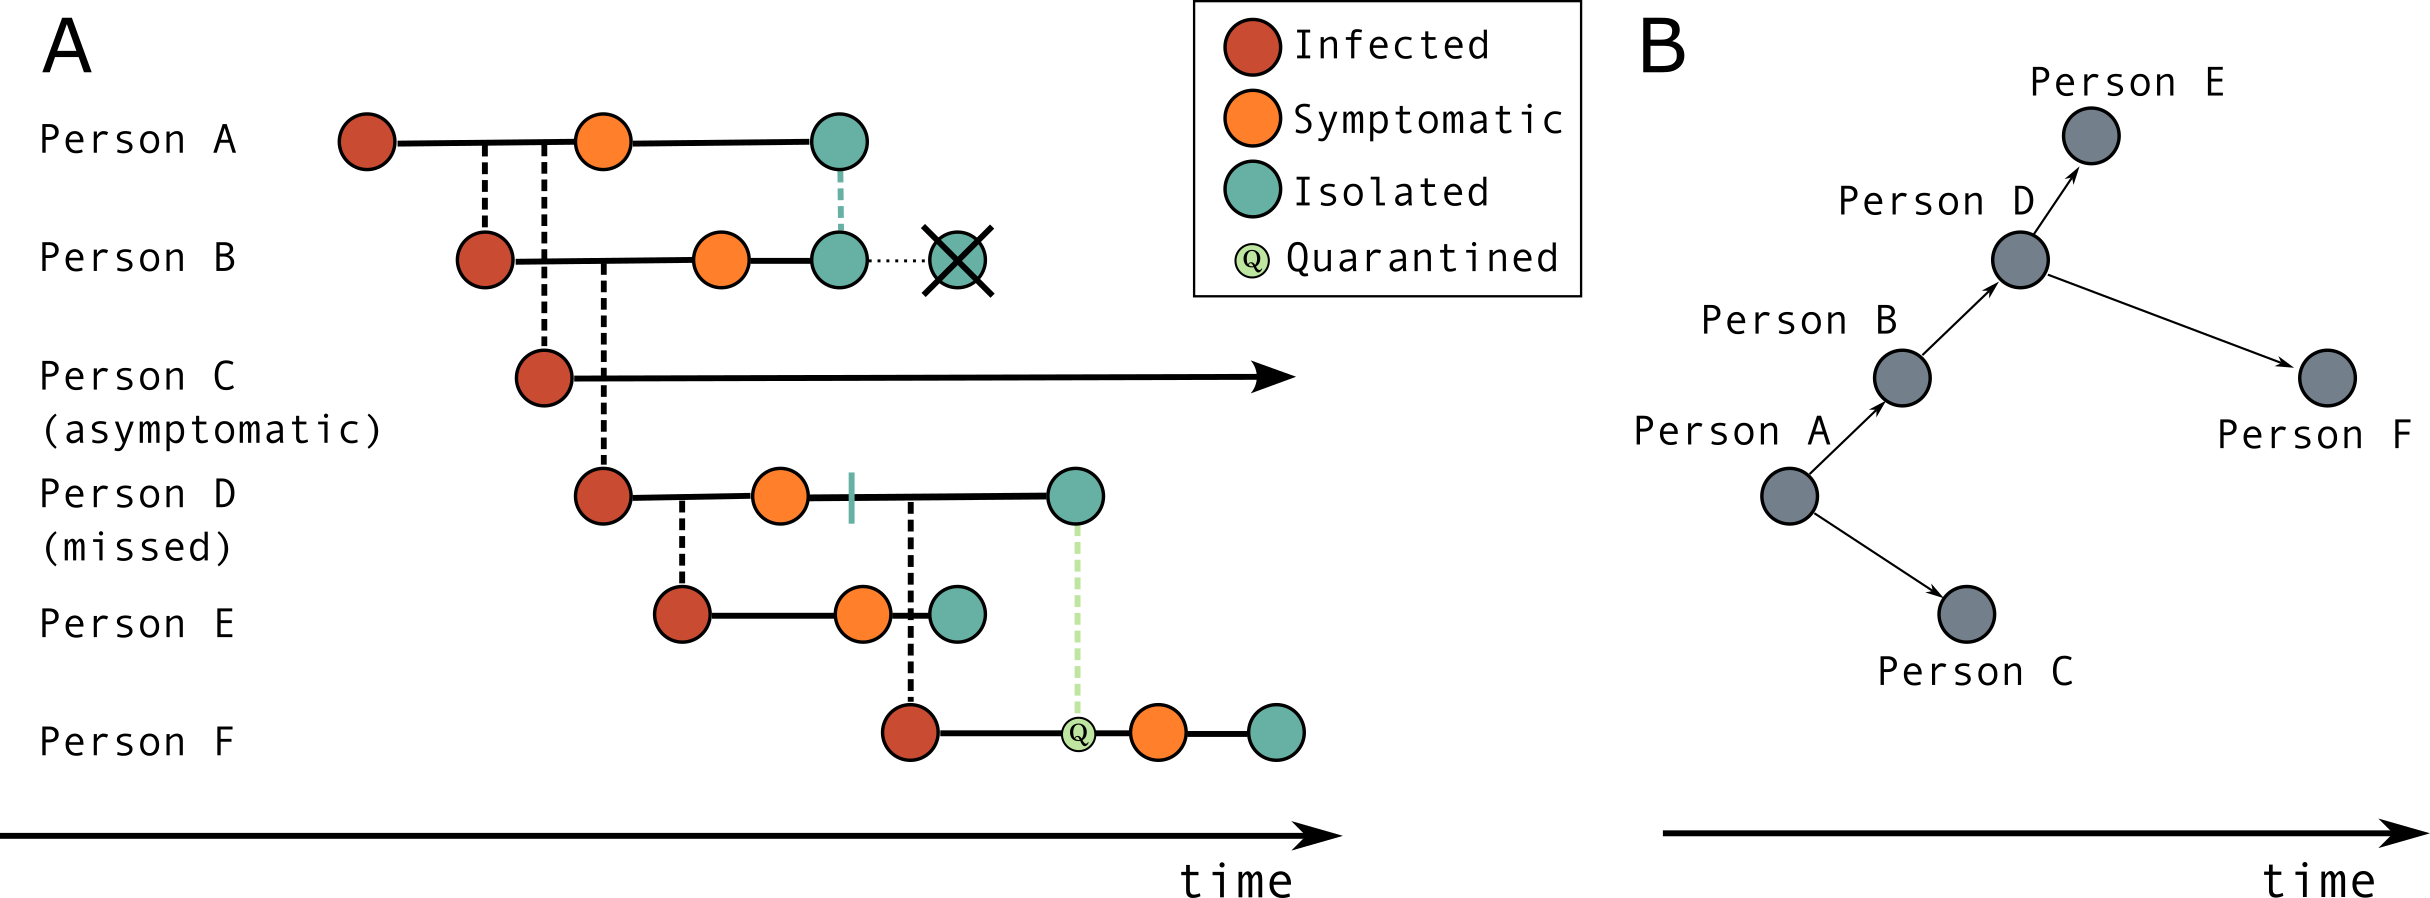
\includegraphics[width=\textwidth]{../plots/model-schematic.png}
\caption{Model schematic of the branching process with isolation, quarantine and contact tracing implemented in the \texttt{\{ringbp\}} R package. (A) The transmission chain from the index case (Person A), infection events are shown by black vertical dashed lines. Individuals can be infected (red circle), become symptomatic (orange circle), and isolated (blue circle). Quarantine is optional in the model, assuming quarantine is active contacts are quarantined when the infector is isolated independent of the contacts symptom status (green circle with Q). The time at which a infectors isolation triggers the isolation of a symtomatic case is shown by the blue vertical dashed line (Person A to Person B). The isolation times that would have been triggered after a delay from symptom onset, but are after isolation was triggered by contact tracing is shown by a blue circle with a cross and connected by a dotted line (Person B). Person C is an asymptomatic individual (asymptomatic cases can infect others). Person D is missed by contact tracing (contacts are traced with a probability $\rho$, and thus missed at $1 - \rho$). The time Person D would have isolated if ascertained is shown by the vertical blue mark. Assuming quarantine is active, Person F would be isolated before symptom onset at the time of the infector's (Person D) isolation time. If quarantine is not active, then Person F would be isolated after a delay from symptom onset, as they had yet to show symptoms when the infector was isolated. (B) A branching process diagram showing who-infected-whom.}
\label{fig:ringbp-model}
\end{figure}

\subsection*{Pathogen epidemiological parameters}

In this study we evaluate the feasibility of controlling outbreaks of A/H5N1-, A/H1N1-, and A/H7N9-like infections. The generation time is modelled using the incubation period and the proportion of presymptomatic transmission to simulate a correlated structure between the two delay distributions to generate sensible delays between exposure, symptom onset and onward transmission (Figure \ref{fig:delay-distributions}A) \citep{hellewellFeasibilityControllingCOVID192020, lintonCorrelationTimesSARSCoV22022}. We extracted previously estimated incubation periods from the literature for each subtype. \cite{nishiuraEstimationIncubationPeriod2011} report the best fitting Weibull shape and scale parameters for H1N1 to be 1.77 and 1.86, respectively (Figure \ref{fig:delay-distributions}B). \cite{cowlingComparativeEpidemiologyHuman2013} report the incubation period for H5N1 and H7N9, both Weibull distributed. For H5N1 the Weibull distribution has a mean of 3.3 days and standard deviation (SD) of 1.5 days, for H7N9 the Weibull distribution has a mean of 3.1 days and SD 1.4 days \citep{cowlingComparativeEpidemiologyHuman2013} (Figure \ref{fig:delay-distributions}B). Comparatively, the incubation period for H1N1 shorter than the other two subtypes (H5N1 and H7N9), which are similar, with H5N1 having a slightly longer median (Figure \ref{fig:delay-distributions}B). \\

We simulated three presymptomatic transmission scenarios: 1\%, 15\%, and 30\% of transmission occurring prior to symptom onset. We assumed that asymptomatic infections can occur and infect others, but are less common that symptomatic infectious indivdiuals and that the majority of cases will develop symptoms during their infectious period.  We ran scenarios with three different assumed proportion of asymptomatic cases, one with zero asymptomatic illness, another with 10\% of cases being asymptomatic and the most extreme scenario where 30\% of cases never develop symptoms and thus are not isolated and secondary cases are missed by contact tracing. These proportions of presymptomatic transmission and asymptomatic fraction cover a broad range of possible pandemic influenza possibilities (Figure \ref{fig:patho-param-space}) \citep{lesslerOutbreak2009Pandemic2009, xuSerologicalInvestigationSubclinical2013, montgomeryRoleAsymptomaticInfections2024, gargHighlyPathogenicAvian2025}. \\

\begin{figure}[ht]
\centering
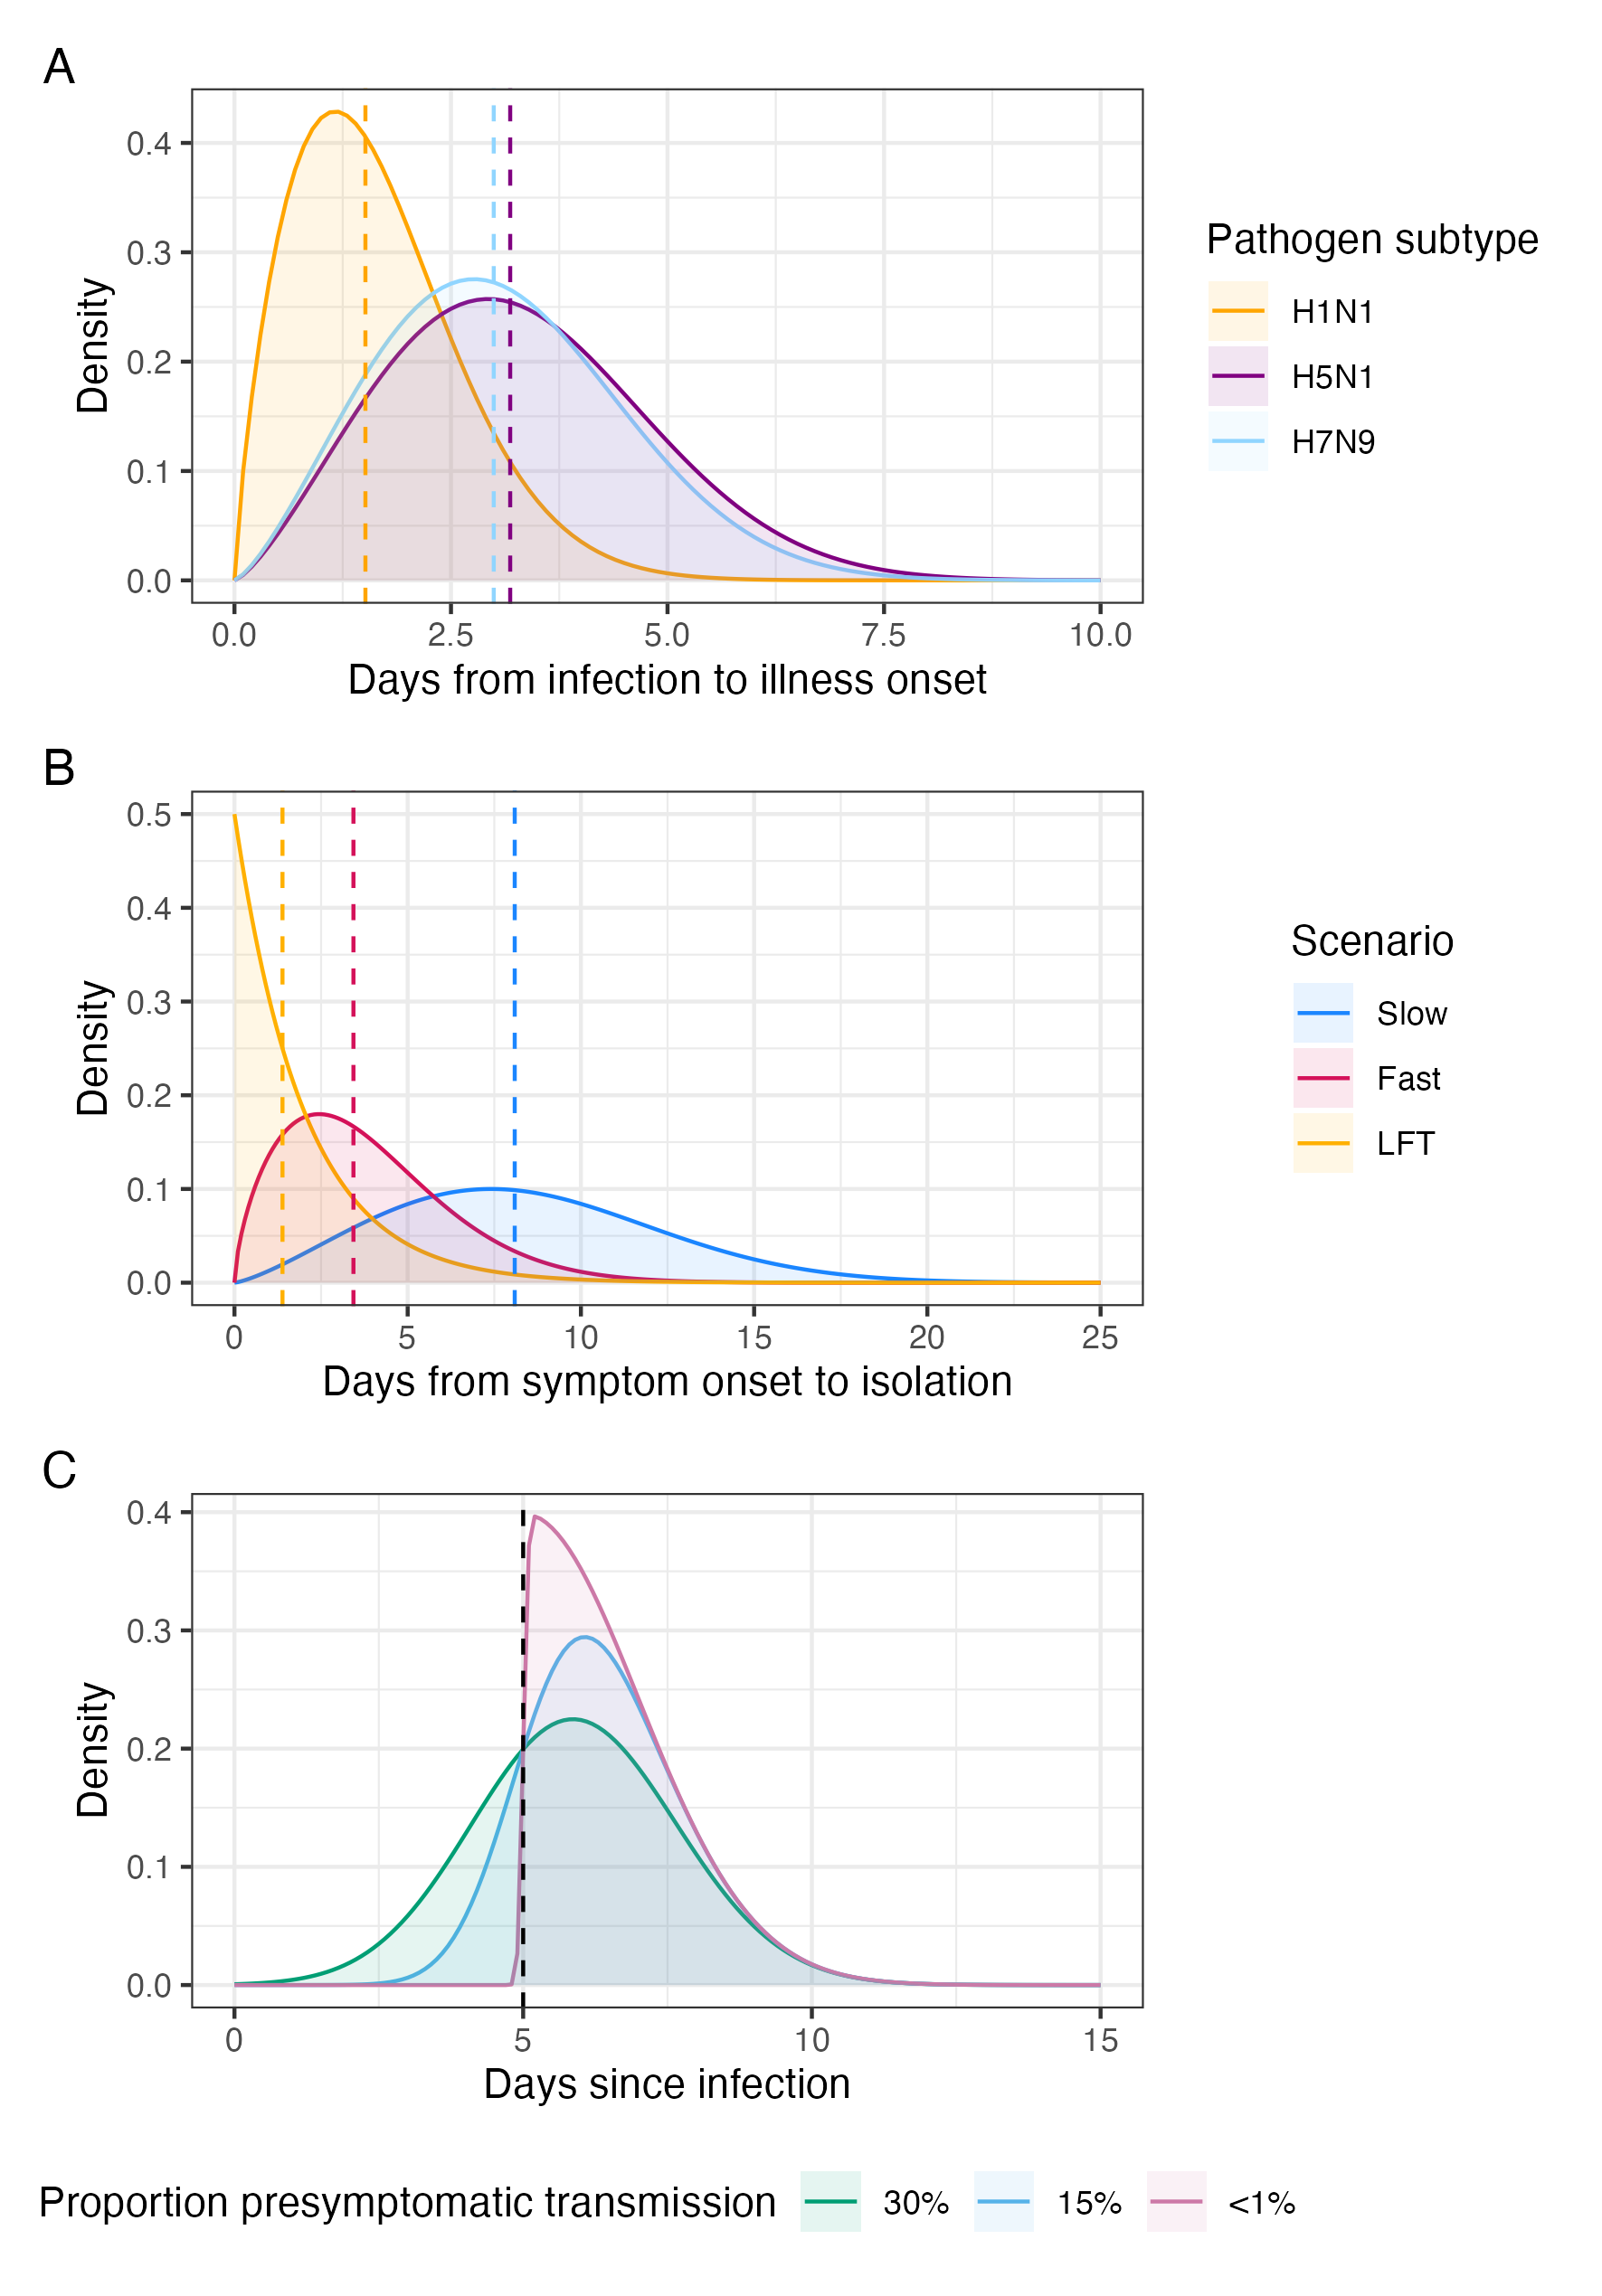
\includegraphics[width=\textwidth,height=0.85\textheight]{../plots/delay_distributions.png}
\caption{(A) Proportion of presymptomatic transmission determined by the incubation period, here assumed to be 5 days (dashed vertical line), controlled by a skew-normal distribution. Three skew-normal distribution probability density functions are plotted with different skew parameters, 0.73, 1.96, 31.82, which correspond to 30\%, 15\% and 1\% presymptomatic transmission. (B) Incubation period for the influenza subtypes: A/H1N1, A/H5N1 and A/H7N9. The vertical dashed lines are the median incubation period: A/H1N1 is 1.5 days (yellow dashed line), A/H5N1 is 3.2 days (purple dashed line), and A/H7N9 is 3.0 days (blue dashed line). (C) Three assumed onset-to-isolation delays used in the simuluation experiment. The \textit{Slow} scenario is based on the onset-to-isolation for the SARS-CoV-2 response in Wuhan, China \citep{liEarlyTransmissionDynamics2020}, the median onset-to-isolation is 8.1 days (blue dashed line). The \textit{Fast} scenario is based on the onset-to-isolation for SARS-CoV-1 response in Hong Kong \citep{donnellyEpidemiologicalDeterminantsSpread2003a}, the median onset-to-isolation time is 3.4 days (red dashed line). The lateral flow test (LFT) scenario is an assumed distributed for rapid self-administered home testing upon isolation, the median delay from symptom onset to isolation in this scenario is 1.4 days (orange dashed line).}
\label{fig:delay-distributions}
\end{figure}

We considered four reproduction number ($R$) values when simulating transmission in the community: 1.1, 1.5, 2.5 and 3.5 (Figure \ref{fig:patho-param-space}). These are based on similar values to previously estimated $R$ values for influenza outbreaks \citep{fergusonStrategiesMitigatingInfluenza2006}, including A/H1N1pdm \citep{fraserPandemicPotentialStrain2009, lesslerOutbreak2009Pandemic2009}, or they represent inflated values of current estimates of A/H5N1 and A/H7N9 subtypes to evaluate the effectiveness of isolation and contact tracing in the event that pathogen evolution enhances the human-to-human transmissibility (e.g. genetic reassortment \citep{peacockGlobalH5N1Influenza2025} or mutations in receptor binding preference \citep{linSingleMutationBovine2024}). Once isolated, cases are assumed to not infect anyone ($R_{iso} = 0$). The reproduction number of asymptomatic cases is assumed equal to the community. The dispersion paramter ($k$) for the negative binomial offspring distributions was fixed at 0.8 for community and asymptomatic cases following evidence that influenza subtypes have moderate transmission heterogeneity \citep{fraserPandemicPotentialStrain2009, heComparingCOVID191918192020, Ward2024.12.11.24318702}.

\begin{figure}[ht]
\centering
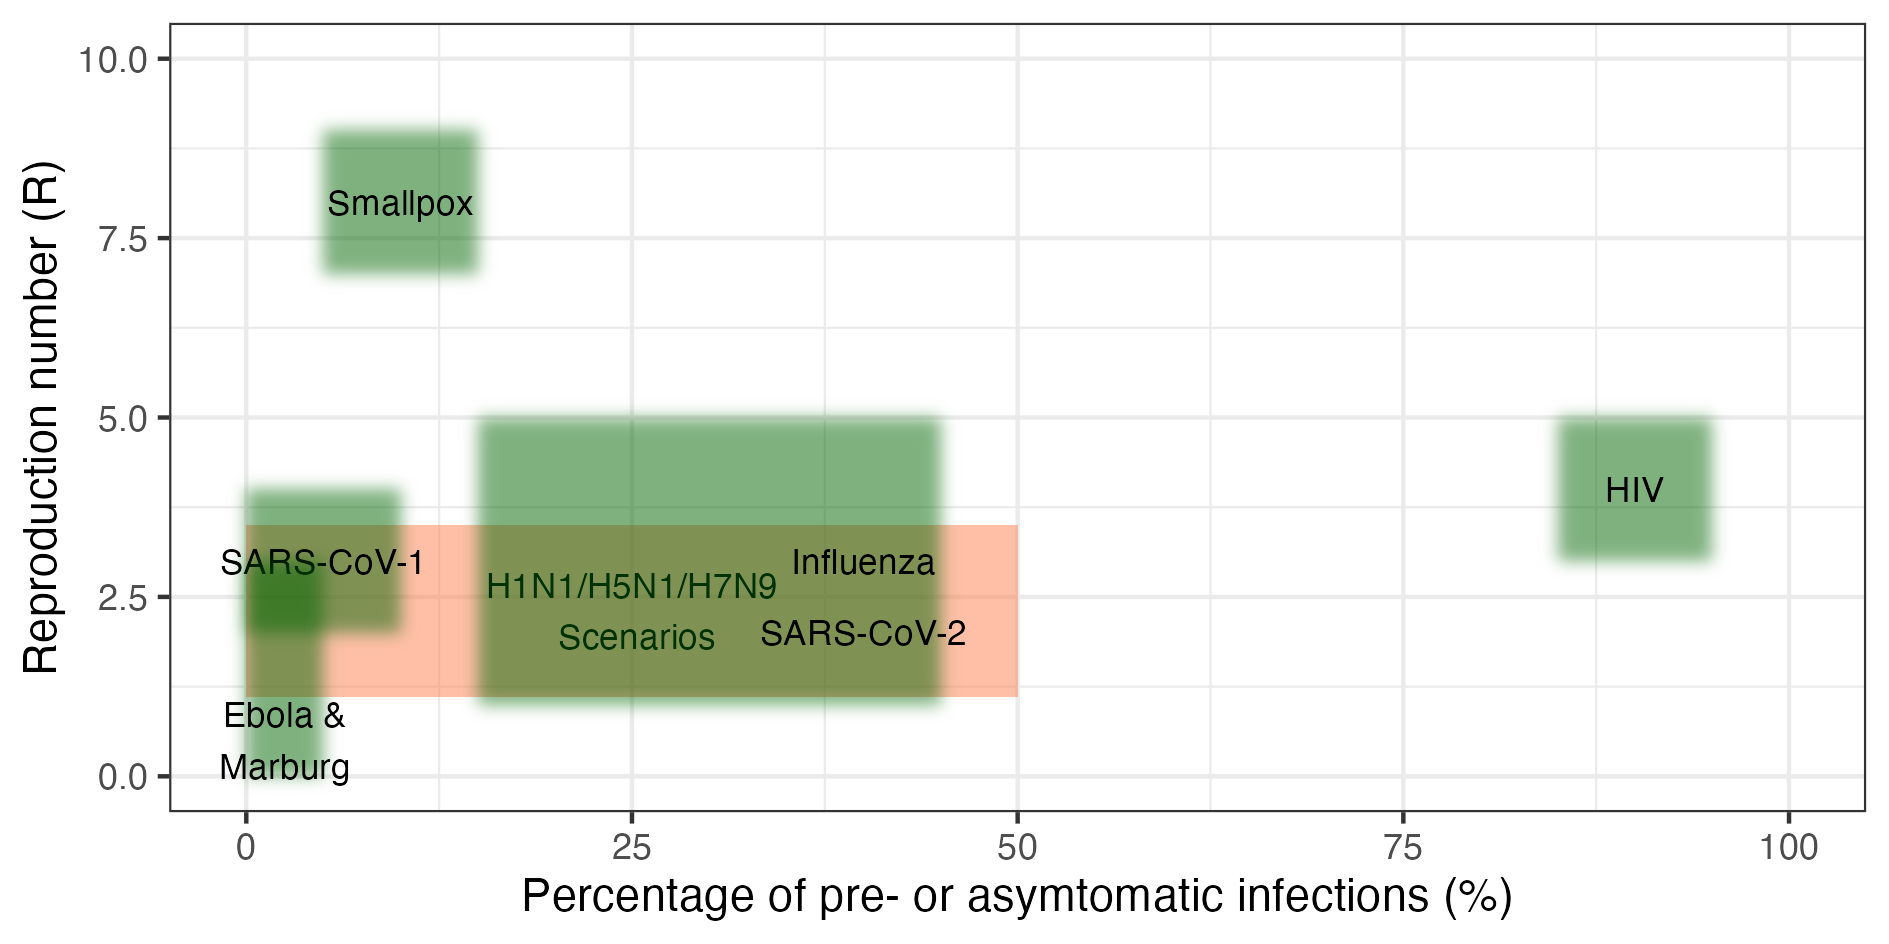
\includegraphics[width=\textwidth]{../plots/patho_param_space.png}
\caption{The pathogen characteristics, in terms of tranmissibility ($R$) and proportion of disease transmission that occurs before the onset of symptoms (including cases that are entirely asymptomatic). The figure includes: Influenza, SARS-CoV-1, SARS-CoV-2, Smallpox, Ebola, Marburg, and HIV shown by green shaded areas. The size of the shaded area reflects the differences in pathogen characteristics, both between variants and outbreaks, the blurred edges reflects uncertainty in parameter estimates. The parameter space of transmissibility and pre- and asymptomatic transmission explored in this paper is shown in the orange box.}
\label{fig:patho-param-space}
\end{figure}

\clearpage

\subsection*{Scenarios}

The onset-to-isolation delay is parameterised under three response scenarios. A fast response, based on the SARS in Hong Kong \citep{donnellyEpidemiologicalDeterminantsSpread2003a} and a slower response based on COVID-19 in Wuhan, China \citep{liEarlyTransmissionDynamics2020} (Figure \ref{fig:delay-distributions}C). Both the fast and slow onset-to-isolation are parameterised as Weibull distributions, the SARS-like distribution has shape ($\lambda$) 1.65 and scale ($k$) 4.29 (mean = 3.83 days, SD = 2.38 days), the COVID-like distribution has shape = 2.31 and scale = 9.48 (mean = 8.40, SD = 3.87 days) (Figure \ref{fig:delay-distributions}C). The third onset-to-isolation scenario is based on a situation where lateral flow rapid tests (LFTs) are provided to all susceptible individuals in the population and these people are freely able to self-test if they are symptomatic. We parameterise this as an exponential distribution, with rate ($\lambda$) 0.5, where most individuals will self-test very shortly after they become symptomatic (approximately 40\% of cases will self-test within the first day of sympmtom onset), with a few people waiting a 2 or more days before testing (approximately 3\% take longer than one week to take a self-test) (Figure \ref{fig:delay-distributions}C). We assume that LFT sensitivity is 100\% accurate so all symptomatic individuals will receive a positive test result. \\

To assess the feasibility of outbreak containment under different proportions of contacts traced and isolated we varied the proportion of contacts ascertained between 0\% (i.e. no contacts traced) and 100\% (i.e. all contacts traced) at intervals of 20\%. When contact ascertainment is zero, isolation is the only NPI reducing transmission. To test scenarios where an outbreak starts with different number of initial infections, we simulate with either 5, 20 or 40 initial independent cases. This could represent importation of multiple cases in a single event, such as a flight. Lastly, we determine if addtionally quarantining contacts, that is isolating contacts once the infector is isoloted independent of whether the contact is symptomatic, improves the ability to contain influenza outbreaks.

\subsection*{Defining outbreak control}

We define outbreak control as no new cases after 12 weeks from the start of an outbreak. The rationale for this criteria is that some outbreaks that do not take off and become sustained may still have cases for the first few weeks of an outbreak, therefore the window for control needs to be enough time after the seeding of an outbreak to be sure it is contained \citep{hellewellFeasibilityControllingCOVID192020}. Due to the exponential dynamics of outbreaks and no depletion of susceptibles in our model we implement a maximum number of cases in each simulation. When this cumulative case limit is reached, it is judged to be a sustained epidemic, not controllable within 12 weeks. We set this limit to 5,000 cases.

\section*{Results}

The reproduction number, contact tracing ascertainment and speed of isolation all affect the ability to control a pandemic potential influenza outbreak (Figure \ref{fig:prop-outbreak-control-R}). Isolation alone can control over 50\% of epidemics with an $R$ of 1.1 with a slow onset-to-isolation response (median 8.1 days); while a fast (median 3.4 days) or LFT (median 1.4 days) response almost always controls $R = 1.1$ outbreaks (Figure \ref{fig:prop-outbreak-control-R}). When $R = 1.5$, $>$75\% of contacts need to be traced to control at least 75\% of outbreaks for a slow onset-to-isolation, whereas only 40\% of contacts require tracing for at least 75\% controlled under a fast isolation delay (Figure \ref{fig:prop-outbreak-control-R}A,B). The isolation upon rapid LFT self-testing controls epidemics with $R \leq 1.5$ without tracing contacts (Figure \ref{fig:prop-outbreak-control-R}C). High transmissibility scenarios ($R \geq 2.5$) require comprehensive contact tracing to contain at least 50\% of simulated outbreaks ($\sim$ 100\% for a slow response and $\sim$ 80-100\% for a fast response). Isolation and tracing 80\% of contacts using LFTs to trigger isolation controls over 80\% of simulated outbreaks for all subtype and transmissibility scenarios (Figure \ref{fig:prop-outbreak-control-R}C). \\

\begin{figure}[ht]
\centering
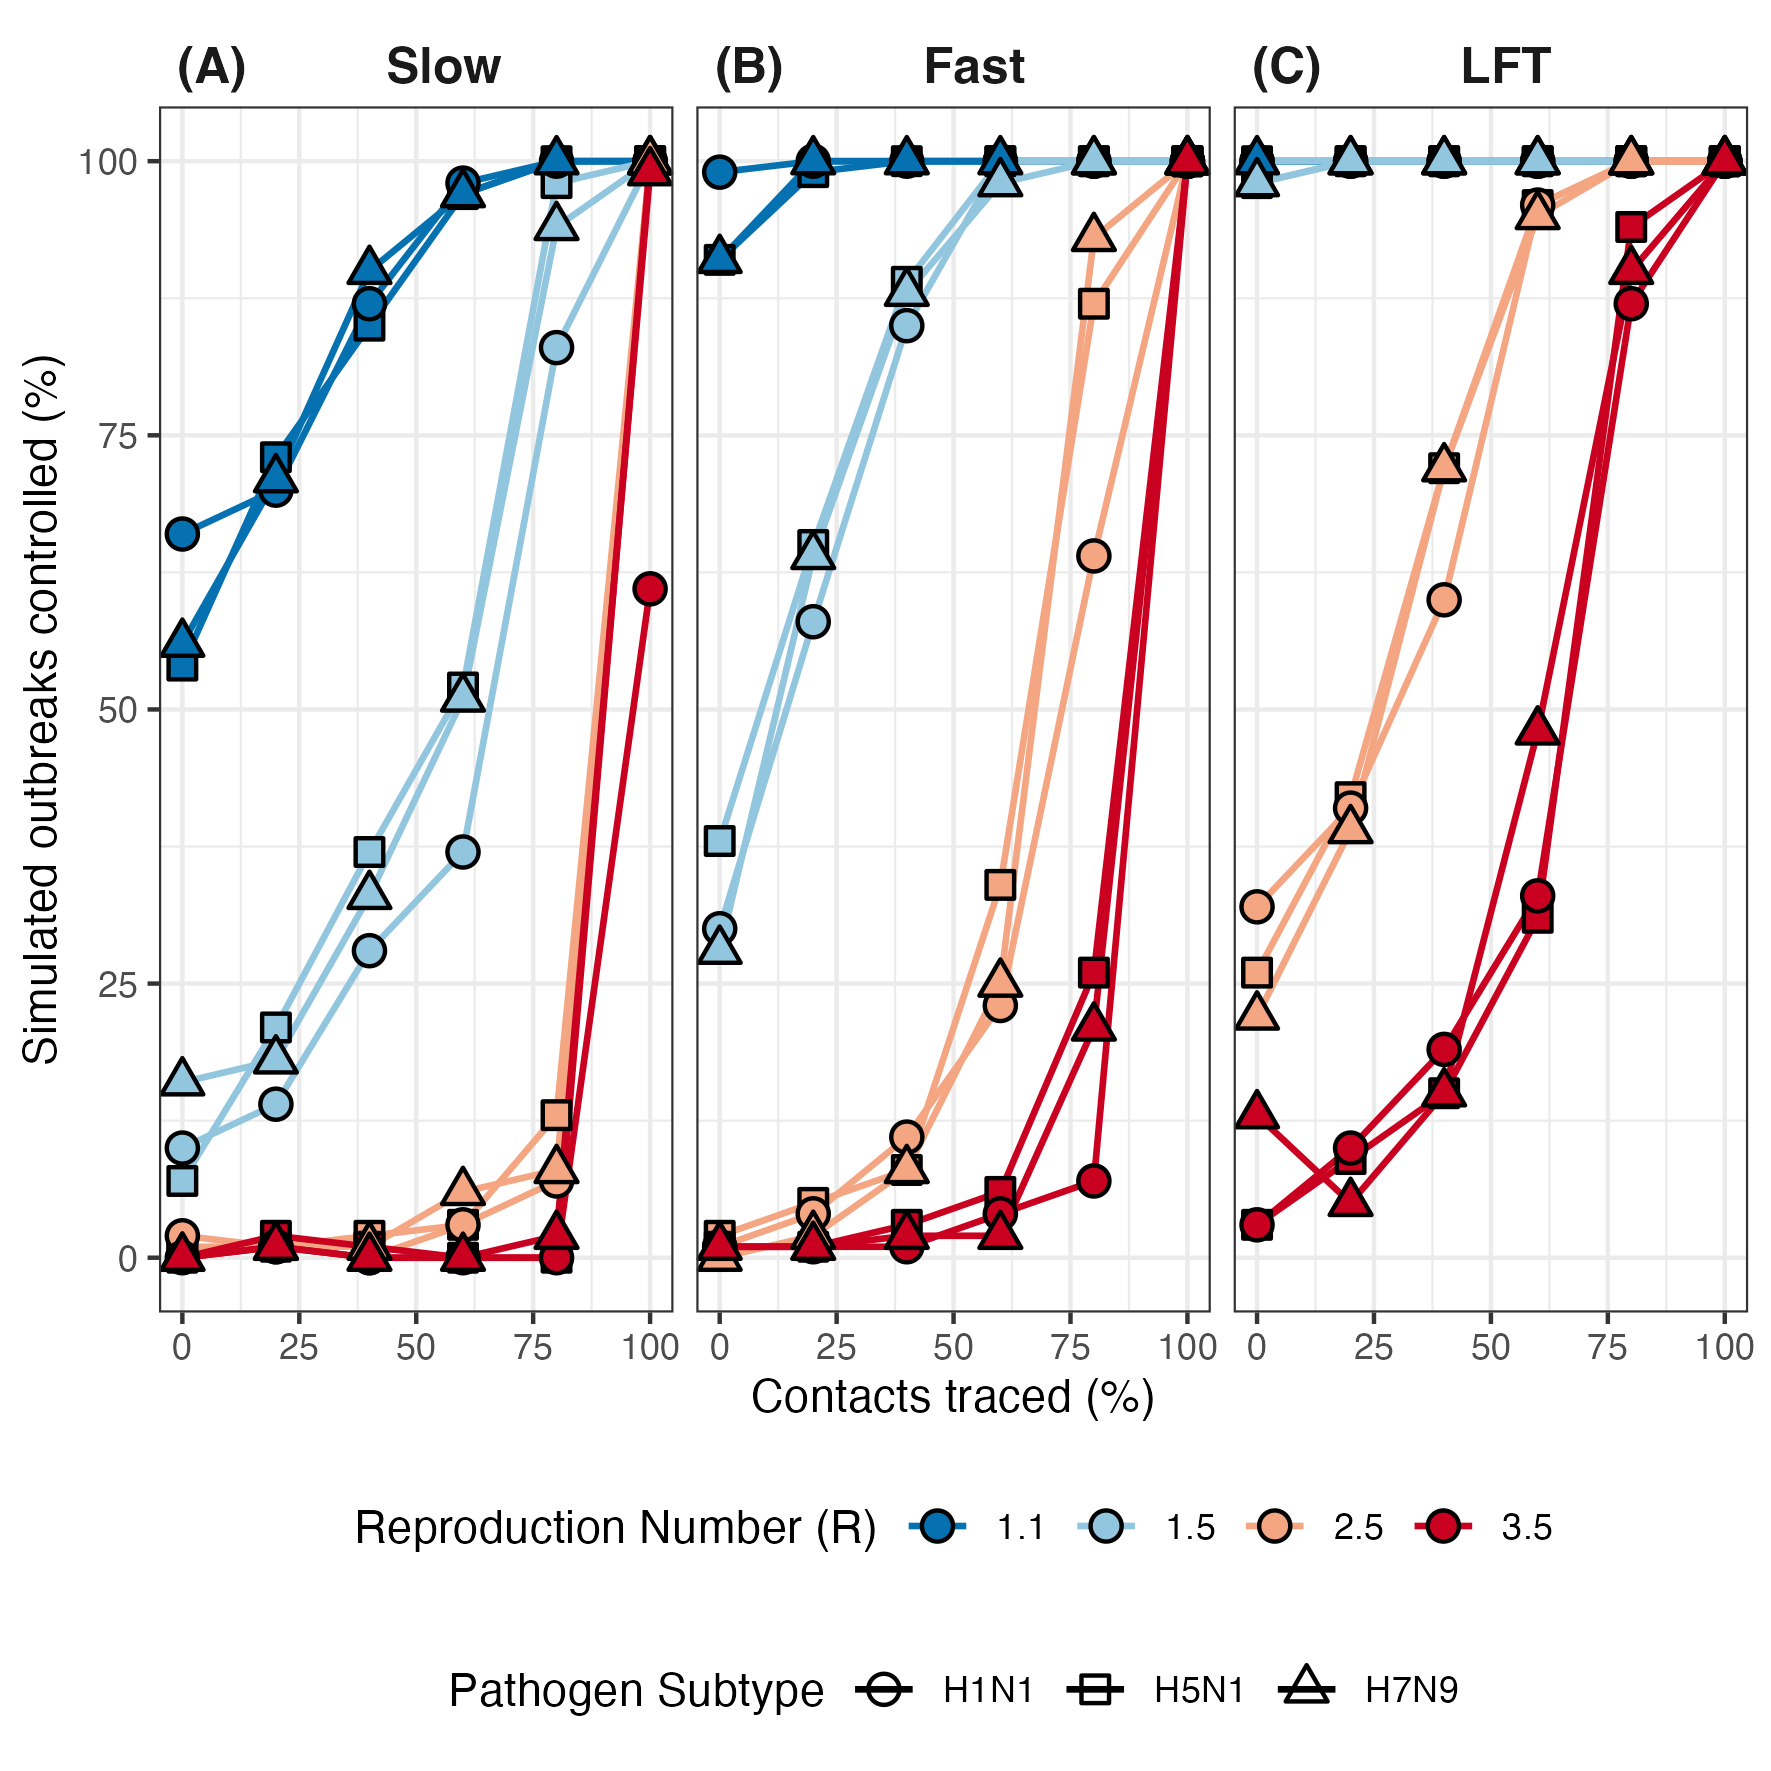
\includegraphics[width=\textwidth]{../plots/prop_outbreak_control_reproduction_number.png}
\caption{The percentage of outbreaks controlled across values of isolation and contact tracing effectiveness, for outbreaks with an assumed reproduction number ($R$) of either 1.1 or 1.5. This is for a baselines scenario where the number of initial cases is 10, the proportion of presymptomatic transmission is 15\%, all cases are assumed symptomatic, and the onset-to-isolation delay is assumed to be SARS-like.}
\label{fig:prop-outbreak-control-R}
\end{figure}

There is some variability in the effectiveness of isolation and contact tracing for outbreak control between influenza subtypes. A/H1N1, because of its shorter incubation period and thus faster tempo of transmission, has a lower proportion of outbreaks controlled, most noticably for $R \geq 1.5$ (Figure \ref{fig:prop-outbreak-control-R}). There is not a strong pattern for the variance in outbreak control between influenza subtypes across scenarios; the few scenarios with higher variance between subtypes are at high percentages of contacts traced ($\geq$ 60\%) and for high transmissibility scenarios (Figure \ref{fig:prop-outbreak-control-var-R}). \\

Increased presymptomatic transmission and asymptomatic cases decreases epidemic containment (Figure \ref{fig:prop-outbreak-control-prop-presym-iso} and \ref{fig:prop-outbreak-control-prop-asym-iso}). When 30\% of transmission occurs before symptom onset, in high transmissibility scenarios ($R \geq 2.5$) more than half of outbreaks become sustained epidemics for all onset-to-isolation delays (Figure \ref{fig:prop-outbreak-control-prop-presym-iso}). When only 1\% of transmission is presymptomatic and contact tracing ascertains all contacts, outbreaks with $R = 3.5$ are contained in $>$75\% of outbreaks with LFT testing, and in $\sim$25\% of outbreaks with a fast isolation response (Figure \ref{fig:prop-outbreak-control-prop-presym-iso}). When all cases develop symptoms, isolation and contact tracing all contacts can control all outbreak scenarios, with the sole exception being A/H1N1 with $R = 3.5$ and a slow onset-to-isolation (Figure \ref{fig:prop-outbreak-control-prop-asym-iso}). When 10\% of cases are asymptomatic the ability to contain highly transmissible influenza ($R \geq 2.5$) dramatically decreases, and decreases further when 30\% of cases are asymptomatic or paucisymptomatic, even with comprehensive contact tracing and isolation upon LFT self-testing, less than a quarter of outbreaks are contained (Figure \ref{fig:prop-outbreak-control-prop-asym-iso}). \\

The more cases that initially seed an outbreak with $R \geq 1$, the less chance that it will stochastically go extinct and we find that the higher the number of initial influenza cases reduces the efficacy of control-by-isolation (Figure \ref{fig:prop-outbreak-control-num-init-cases}). Isolation alone can control outbreaks with $R = 1.1$ even when seeded with 40 initial cases (Figure \ref{fig:prop-outbreak-control-num-init-cases}). When $R \geq 1.5$ increasing the number of initial cases makes epidemics less controllable for all influenza subtypes. For high transmissibility ($R \geq 2.5$) scenarios that are seeded with at least 20 cases, close to 100\% of contacts need to be traced and isolated upon symptom onset to control the majority of outbreaks, assuming a fast onset-to-isolation response (3.4 days on average) (Figure \ref{fig:prop-outbreak-control-num-init-cases}). \\

\begin{figure}[ht]
\centering
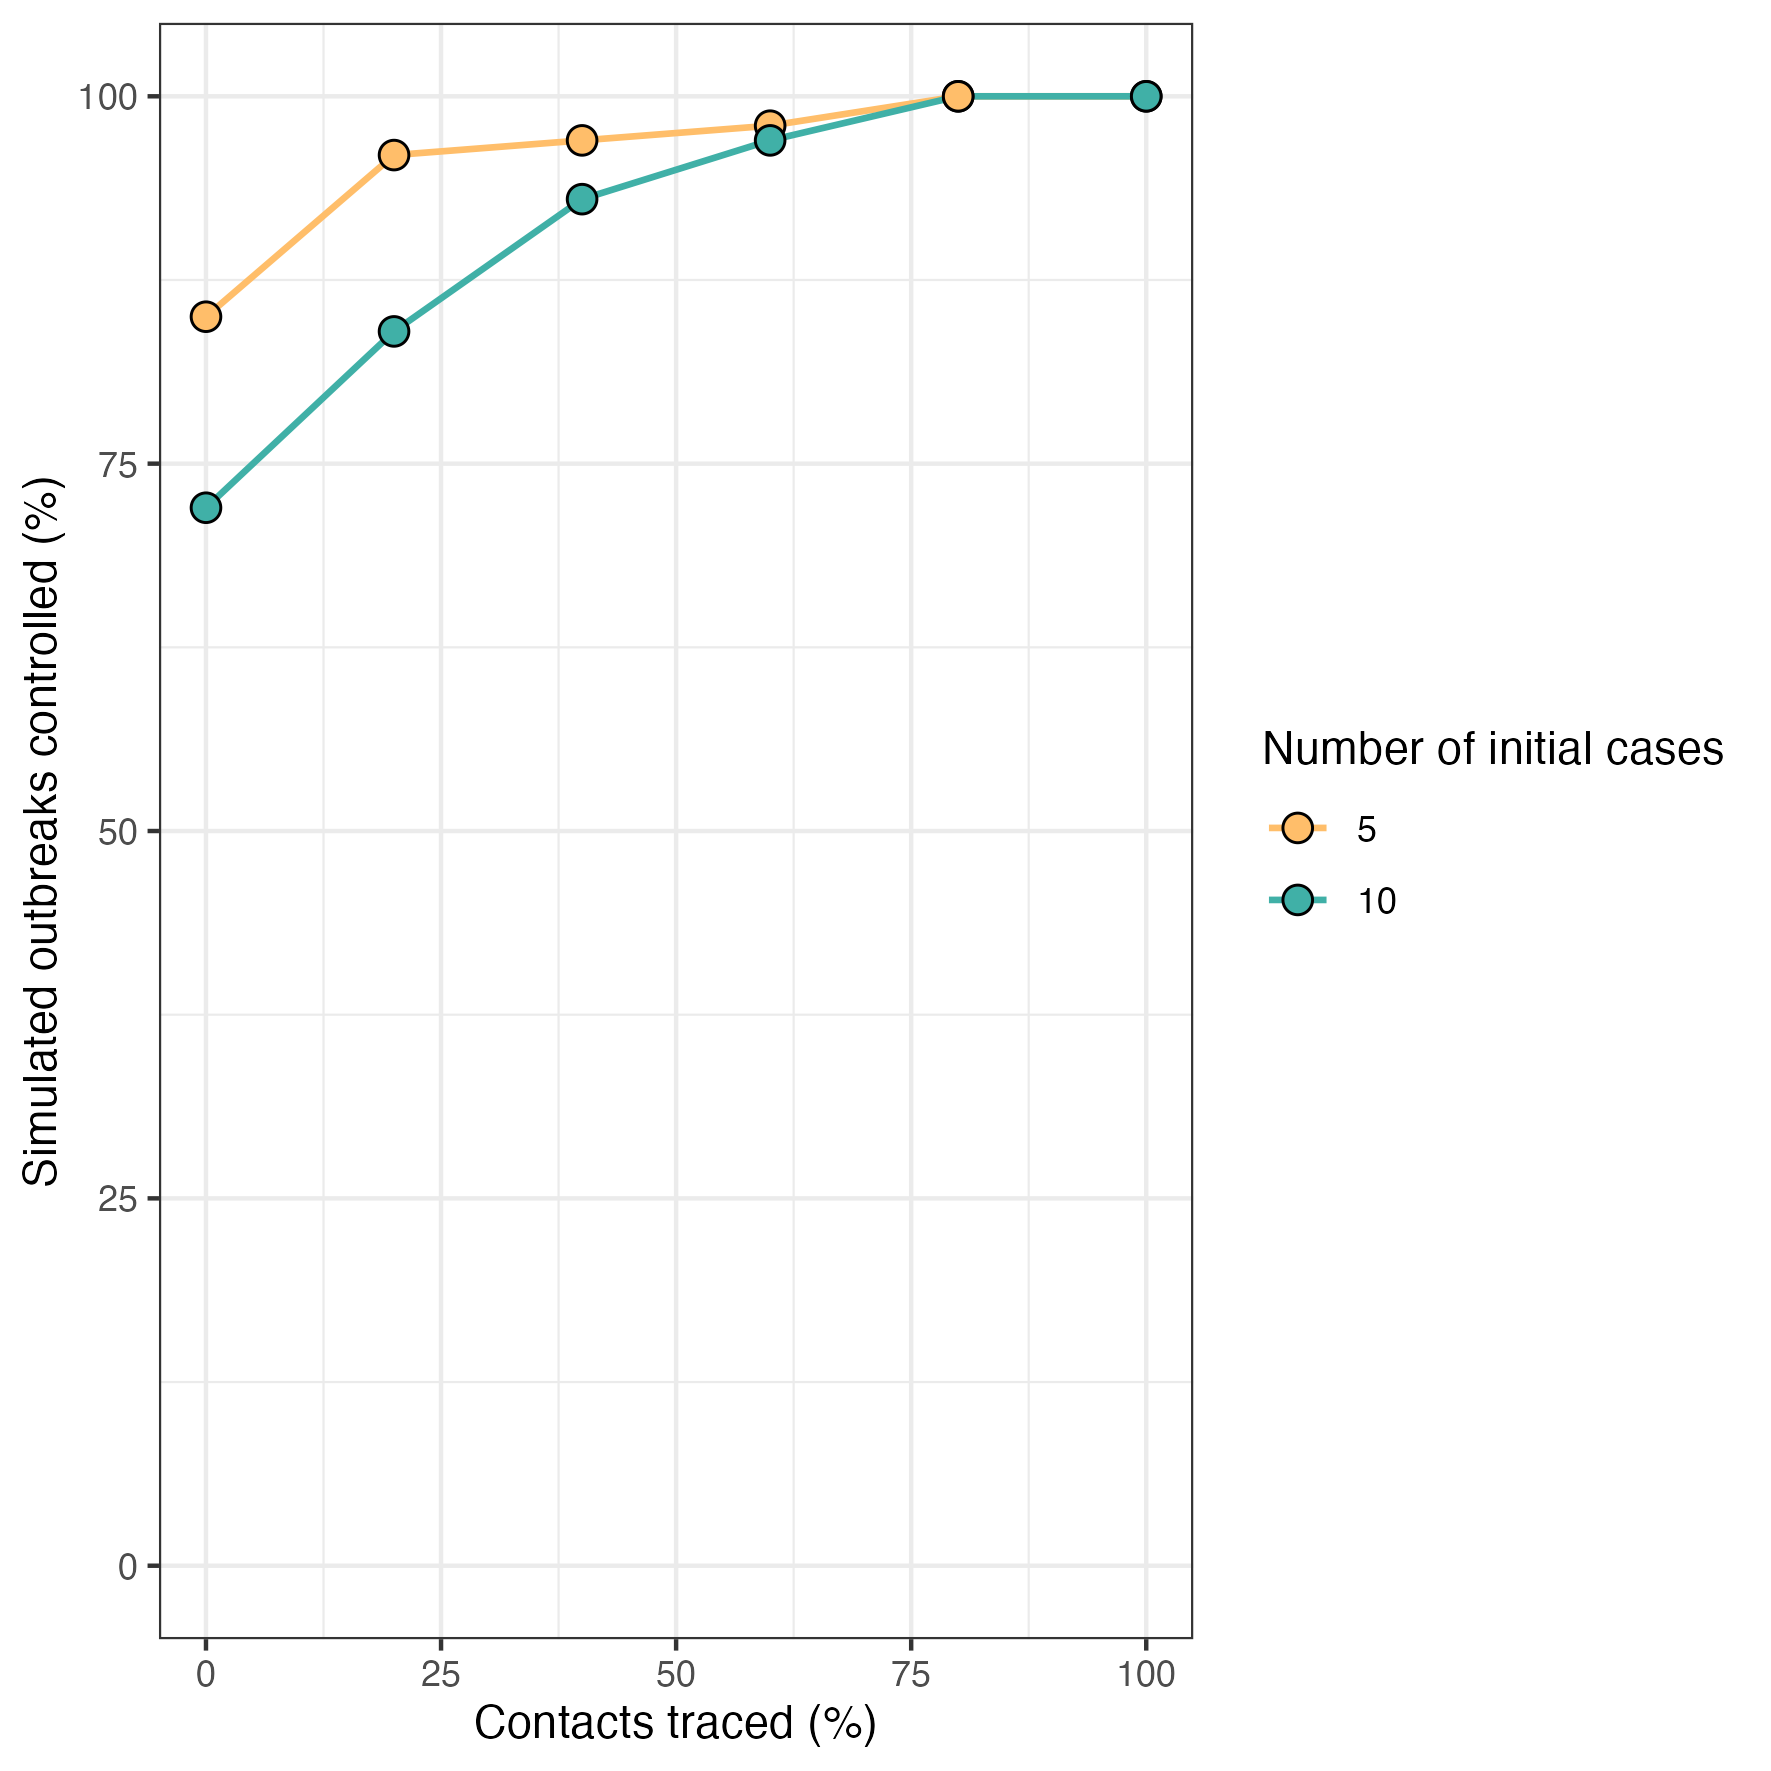
\includegraphics[width=\textwidth]{../plots/prop_outbreak_control_num_init_cases.png}
\caption{The percentage of outbreaks controlled across values of isolation and contact tracing effectiveness, for outbreaks with an initial number of seeding infections assumed to be either 5 or 10. This is for a baselines scenario where the reproduction number is 1.5, the proportion of presymptomatic transmission is 15\%, all cases are assumed symptomatic, and the onset-to-isolation delay is assumed to be SARS-like.}
\label{fig:prop-outbreak-control-num-init-cases}
\end{figure}

In the acute phase of outbreaks there can be thousands of weekly cases, especially for high transmissibility scenarios ($R \geq 2.5$) (Figure \ref{fig:max-weekly-cases}). Specifically for controlled outbreaks, the cumulative number of cases is consistently below 500 cases across influenza subtypes (Figure \ref{fig:median-controlled-outbreak-size}). Thus when an outbreak is controlled with isolation alone or in combination with contact tracing it is done so without incurring a high initial prevalence. \\

The control of influenza outbreaks with a $R > 1$ require interventions to bring $R$ below 1 for transmission to eventually cease. Isolation of symptomatic cases alone reduces $R$ (Figure \ref{fig:r0_low_presym_asym}). When the delay between symptom onset and isolation is around 8 days (i.e. slow response), the reduction in $R$ can be minimal, whereas if isolation is rapid after symptom onset, around 1.5 days (i.e. LFT self-testing response), isolation without contact tracing or quarantine brings $R_t$ below 1 when $R_0 < 3$ (Figure \ref{fig:r0_low_presym_asym}). Contact tracing can further suppress transmission, with 100\% contact ascertainment bringing an outbreak under control ($R < 1$) for all influenza subtypes and isolation responses for $R_0 < 2.5$ (Figure \ref{fig:r0_low_presym_asym}). Quarantine has a negligible impact on the reducing disease transmission, with a slightly greater reduction in transmission when there is a higher proportion of presymptomatic transmission (Figure \ref{fig:r0_low_presym_asym} and \ref{fig:r0_high_presym_asym}). The effectiveness of tracing and isolating contacts is reduced when more cases transmit before symptomatic or are asymptomatic (Figure \ref{fig:r0_low_presym_asym} and \ref{fig:r0_high_presym_asym}).

\begin{figure}[ht]
\centering
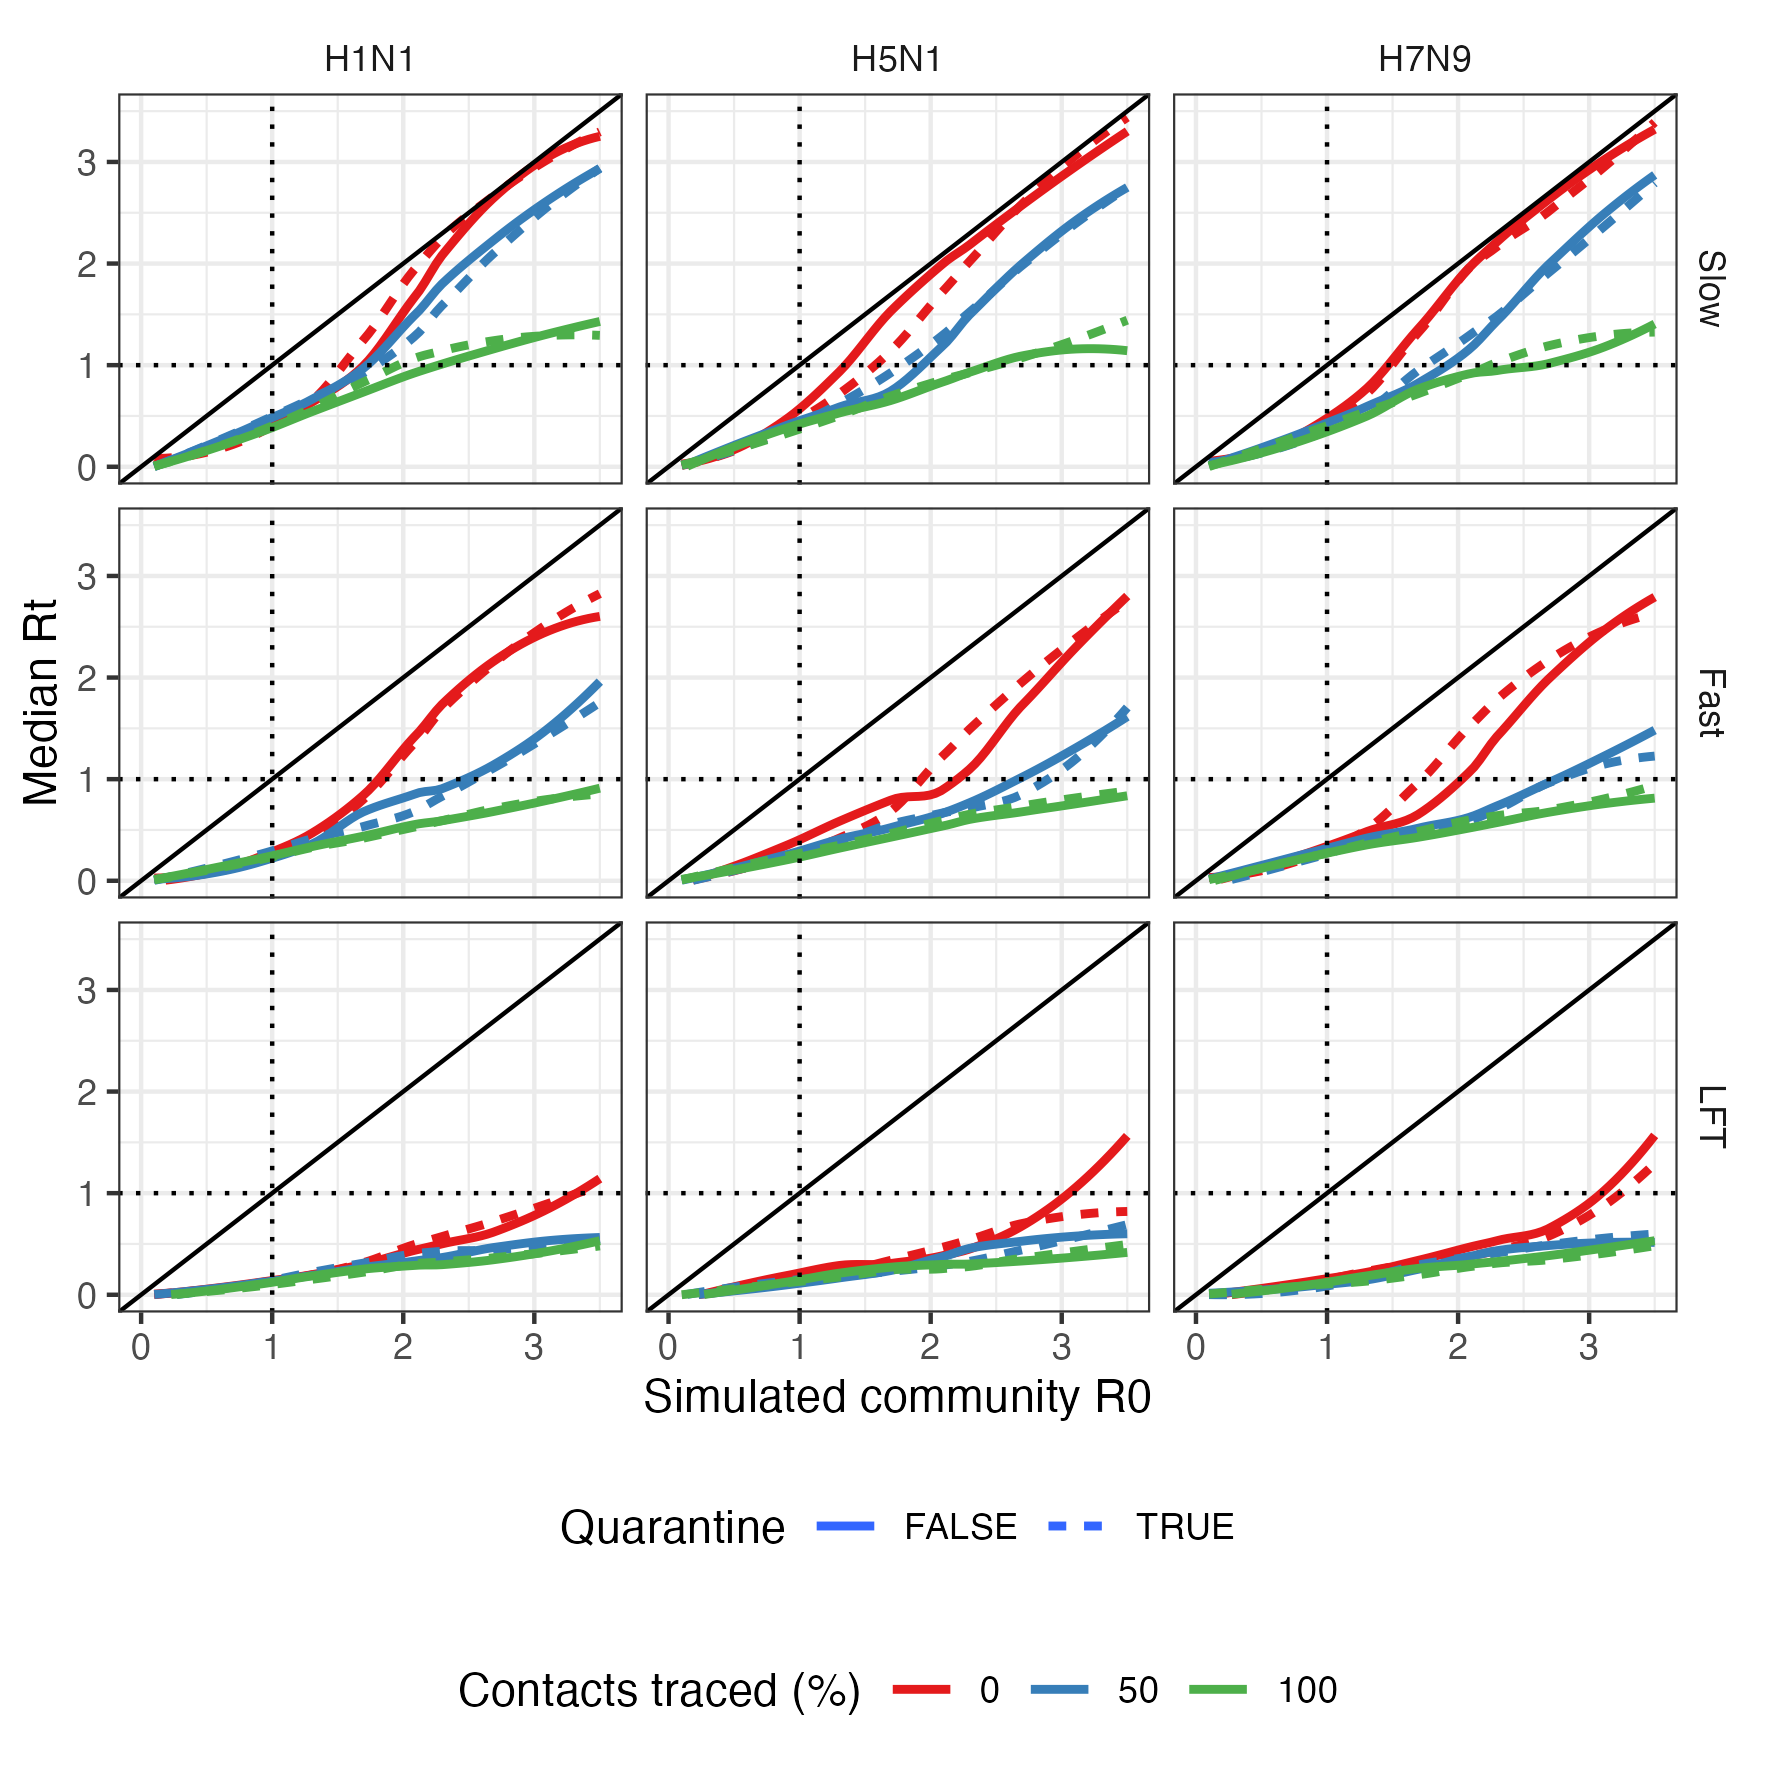
\includegraphics[width=\textwidth]{../plots/r0_low_presym_asym.png}
\caption{The median effective reproduction number ($R_t$) across simulation replicates calculated from simulated outbreak data under various influenza subtype and intervention scenarios against the basic reproduction number ($R_0$) for the general community used to simulate the outbreaks. The $R_0$ value for isolated cases is zero. The diagonal line shows an equal value for $R_t$ and community $R_0$. The dotted lines are where the values of $R_t$ (horizontal) or community $R_0$ (vertical) equal unity. Values of $R_t$ below the diagonal indicate a reduction in transmission from NPIs compared to uncontrolled community transmission. Isolation of symptomatic cases is active for all scenarios, contact tracing ascertainment is plotted for 0\% (no contact tracing), 50\% and 100\% (all symptomatic contacts of symptomatic cases traced), we run each scenario with quarantine of contacts active (dashed line) and inactive (solid line). This is for a baseline scenario where the proportion of presymptomatic transmission is 1\% and the proportion of asymptomatic cases is 0\%.}
\label{fig:r0_low_presym_asym}
\end{figure}

\clearpage

\section*{Discussion}

Influenza remains a high risk pathogen with pandemic potential as shown by the history of influenza pandemics throughout the 20th century \citep{saunders-hastingsReviewingHistoryPandemic2016}. The recent spread of A/H5N1 avian influenza in cattle and poultry farms, primarily in the US, creates a greater spillover risk and adaptations to enhance mammal-to-mammal transmission \citep{linSingleMutationBovine2024, gargHighlyPathogenicAvian2025, peacockGlobalH5N1Influenza2025}. In this study we use a mathematical model to assess the feasibility and effectiveness of isolation and contact tracing for avian and non-avian influenza subtypes to determine whether these should be considered effective NPIs in the event that sustained human-to-human transmission is detected. \\

We find that the percentage of contacts that need to be successfully traced to control an outbreak depends on the reproduction number of the pathogen, and the speed at which a public health system can respond by testing and communicating with those infected and contacts of infectious persons. If the delay between symptom onset and isolation is at least one week, then isolation and comprehensive contact tracing are required to be confident a moderate to highly transmissible ($R \geq 1.5$) influenza can be controlled. By reducing the delay between symptom onset and isolation to around three days, influenza pathogens that are marginally supercritical ($R = 1.1$) become subcritical ($R < 1$) and contained by isolation alone, and more transmissible scenarios can be controlled with good contact tracing coverage. In addition to two empirically-based onset-to-isolation delays, by testing a rapid isolation scenario where LFTs that do not require a test being sent to a laboratory, as would be the case for polymerase chain reaction (PCR) testing, the benefit to containment probability, and the opportunity to control highly transmissible ($R \geq 2.5$) respiratory diseases with isolation and contact tracing. Therefore, the dogma that symptom-based isolation and contact tracing are not effective for influenza is shown not to hold for optimal testing and isolation scenarios, even if some cases are missed due to being asymptomatic and some transmission occurs prior to symptom onset. If making LFTs widely accessible is economical relative to the cost of mass contact tracing, a low to moderate transmissibility influenza pandemic response should focus on reducing the onset-to-isolation response. Whether the interventions proposed here are cost-effective remains a question for further investigation. \\

The transmission model highlights the bimodal nature of the final size of outbreaks, where NPI-controlled epidemics typically range from tens to hundreds of total cases, in contrast, uncontrolled outbreaks can produce thousands of new cases each week. The severity of avian influenza subtypes is uncertain, historical estimates are $\sim$30\% --- 55\% \citep{tannerPandemicPotentialAvian2015}, but recent human infections have lower morbidity and mortality \citep{gargHighlyPathogenicAvian2025, krammerHighlyPathogenicAvian2025}. Consequently, the difference in disease burden between containing an outbreak while still small compared to allowing thousands of cases will be substantial. Even if updated severity estimates are significantly lower, widespread infections could still result in a devastating outcome. \\

It is possible that a sentinel surveillance system or community testing to detect new cases of pandemic potential influenza (e.g. A/H5N1 or A/H7N9), could miss the primary case(s), whether originating from zoonotic spillover or importation. We show that more cases before an NPI is activated hinders the ability to effectively contain the outbreak. The magnitude of this impact is moderated more by transmissibility than influenza subtype for the three variants we considered. If interventions are activated when case prevalence exceeds 50 cases, then even rapidly isolating over 60\% of people with 2 days of becoming symptomatic will require near-perfect contact tracing coverage. For comparison, on the date of the first fatality in the UK from COVID-19 there were already over 100 confirmed cases and probable sustained widespread community transmission. A subcritical influenza outbreak could cause transient epidemics, during which, adaptation to enhance human-to-human tranmsmission can cause a critical transission to supercritical transition, at which point more importations exponentially decreases containment without interventions \citep{whittleOutcomeStochasticEpidemicA1955, farringtonDistributionTimeExtinction1999, antiaRoleEvolutionEmergence2003, lloyd-smithSuperspreadingEffectIndividual2005}. This study does not model this transition, instead we assume supercritical human-to-human transmission potential for A/H5N1 and A/H7N9 to evaluate NPIs because current estimates for pathogen epidemiology ($R < 1$) do not require interventions for containment. Cases detected with routine surveillance without a known animal source may indicate sustained human-to-human transmission and could be a trigger to commence isolation and contact tracing while the number of initial cases is presumed small. \\

The strength of our approach is based on the simple parameterisation of the individual-based model to capture the infectiousness, disease progression and onward transmission incorporating individual-level heterogeneity. Sampling the generation time using the incubation period and proportion of presymptomatic infections (using a skew-normal distribution) enables simulating transmission dynamics for novel pathogens and early in outbreaks when the incubation period is estimated but the generation time is unknown or estimated with more uncertainty, and the serial interval would introduce bias if used instead \citep{brittonEstimationEmergingEpidemics2019a, lehtinenRelationshipSerialInterval2021}. \\

The model and simulation experiment has several limitations. We assumed that the LFT rapid tests are accurate and do not provide false negatives, in reality these type II errors will result in a smaller reduction in transmission \citep{petoCOVID19RapidAntigen2021}. Secondly, the isolation of infectious individuals is assumed to prevent all onward transmission. This may be overly conservative if for example individuals isolate at home while living with others, who may become infected and continue to spread the disease until they become symptomatic and isolate. We find that quarantine has a negligible reduction -- and counter intuitively in some cases a small increase -- in reproduction number. This is likely due to the model implementation of quarantine, whereby ..., and should not be concluded that quarantine is ineffective for respiratory pathogens. Lastly, the transmission model does not take into account network or age structure which has been shown to influence the effectiveness of isolation and contact tracing (Juul and Strogatz, 2023). \\

We assessed the benefit of contact tracing across a range of possible contact ascertainment levels. In doing so we model up to 5,000 cases before terminating a simulated outbreak as uncontained, but before reaching the case limit we assume that there is no capacity limit on contact tracing. This is an optimistic assumption; in reality surveillance systems can be patchy and have finite capacity, exacerbated in resource-limited settings \citep{dhillonWhenContactTracing2018}. The scenarios where a low percentage of contacts were traced may be more representative for these situtations. The finding that weekly case incidence can reach thousands of new cases within the acute phase of an influenza outbreak highlights how the exponential dynamics of outbreaks, even in the presence of NPIs, can overburden surveillance systems with the volume of testing and isolation required. Aside from public health surveillance capacity, we also ignore potential socio-political factors that may prevent contacting infected individuals or contacts of infected individuals \citep{dhillonWhenContactTracing2018}. In this study we assume that contacts are known, avoiding the need to define what constitutes a contact. In reality the threshold for duration and distance of a contact for a directly transmitted respiratory disease will influence the ascertainment and volume of contact tracing required by balancing the error rates of contacts that result in infections \citep{keelingEfficacyContactTracing2020}. \\

The experience of contact tracing from the COVID-19 pandemic has shown that isolating and quarantining contacts can be expedited with the use of digital tracing. As opposed to symptom-based testing and isolating, a contact can be determine by proximity and duration between mobile devices, and if someone tests positive it can immediately notify all recent contacts \citep{ferrettiQuantifyingSARSCoV2Transmission2020}. This approach would be complimentary to the LFT scenario in this study where available rapid tests could be used when notified of an infectious contact (assuming the time between exposure and testing is longer than the detectable latent period). Decentralising contact tracing to devices most people carry around at all times (e.g. smartphones) would also ease capacity limitations of a centralised contact tracing unit. The optimistic scenarios of traditional testing, tracing and isolating included could in theory be improved and epidemic prevention enhanced by integrating digital technology. \\

Enacting isolation and contact tracing and other NPIs is expected with the emergence of a novel pathogen due to widespread susceptibility and no pharmaceutical interventions. However, influenza has multiple circulating seasonal subtypes and past pandemics, resulting in a complex mosaic of population immunity for different influenza subtypes, with possible immunological imprinting \citep{gosticPotentProtectionH5N12016}. There is also seasonal vaccination availability in many high- and middle income countries \citep{goldinSeasonalInfluenzaVaccination2024}, stockpiles of vaccines for avian influenza, as well as licensed effective antivirals \citep{krammerHighlyPathogenicAvian2025}. We show that asymptomatic influenza infectious will detrimentally influence containment with symptom-based isolation and contact tracing. If an epidemic is highly asymptomatic ($>25$\% cases), countries with a stockpile of influenza antivirals, could deploy those prophylactically in response \citep{haydenPerspectivesAntiviralUse2001}. For example, the UK which stockpiles antivirals for $\sim$ 50\% of the population \citep{WrittenQuestionsAnswers}. Pandemic response could deploy pharmaceutical and non-pharmaceutical interventions in combination to prevent disease burden by suppressing transmission and severity. The stockpile of vaccines for A/H5N1 that shows cross-reactivity with current 2.3.4.4b strain are another line of defence \citep{khuranaLicensedH5N1Vaccines2024}. The speed of isolating contacts compared to vaccinating them in the context of a fast generation time and proportion of presymptomatic transmission, renders a ring vaccination less effective \citep{kucharskiEffectivenessRingVaccination2016, whittakerQuantifyingImpactBroadly2024}. Overall, the response to an influenza pandemic from an avian or swine subtype would be more multifacetted than the baseline containment results from our model. \\

Our study shows that isolation and contact tracing are effective NPIs that should be considered when evaluating a robust outbreak reponse to pandemic potenial influenza. If responding to a pathogen where human-to-human transmission is sustained ($R \leq 1.5$) isolation of symptomatic cases alone will bring the reproduction number below one, and comprehensive tracing and isolation of contacts with a short delay to isolation can control outbreaks with $R \leq 3.5$. Whether the next public health emergency is from avian (A/H5N1 and A/H7N9) or swine (A/H1N1) influenza, the response should be broadly similar. If in the acute phase of the outbreak clinical and epidemiological investigation indicate presymptomatic transmission or asymptomatic infections \citep{liuContributionPresymptomaticInfection2020}, or that multiple imported cases have seeded human-to-human transmission chains \citep{russellEffectInternationallyImported2021}, then increasing contact tracing ascertainment and reducing the onset-to-isolation delay will improve chances of containment. Our results broadly cover to novel emerging pathogens that lack pharmaceutical interventions; extending results to other pandemic pathogen candidates depends on the similarity of their epidemiological characteristics.

\bibliographystyle{plainnat}
\bibliography{FluTracer.bib}

\clearpage

\section*{Supplementary Material}

\setcounter{figure}{0}
\renewcommand{\thefigure}{S\arabic{figure}}


\begin{figure}[ht]
\centering
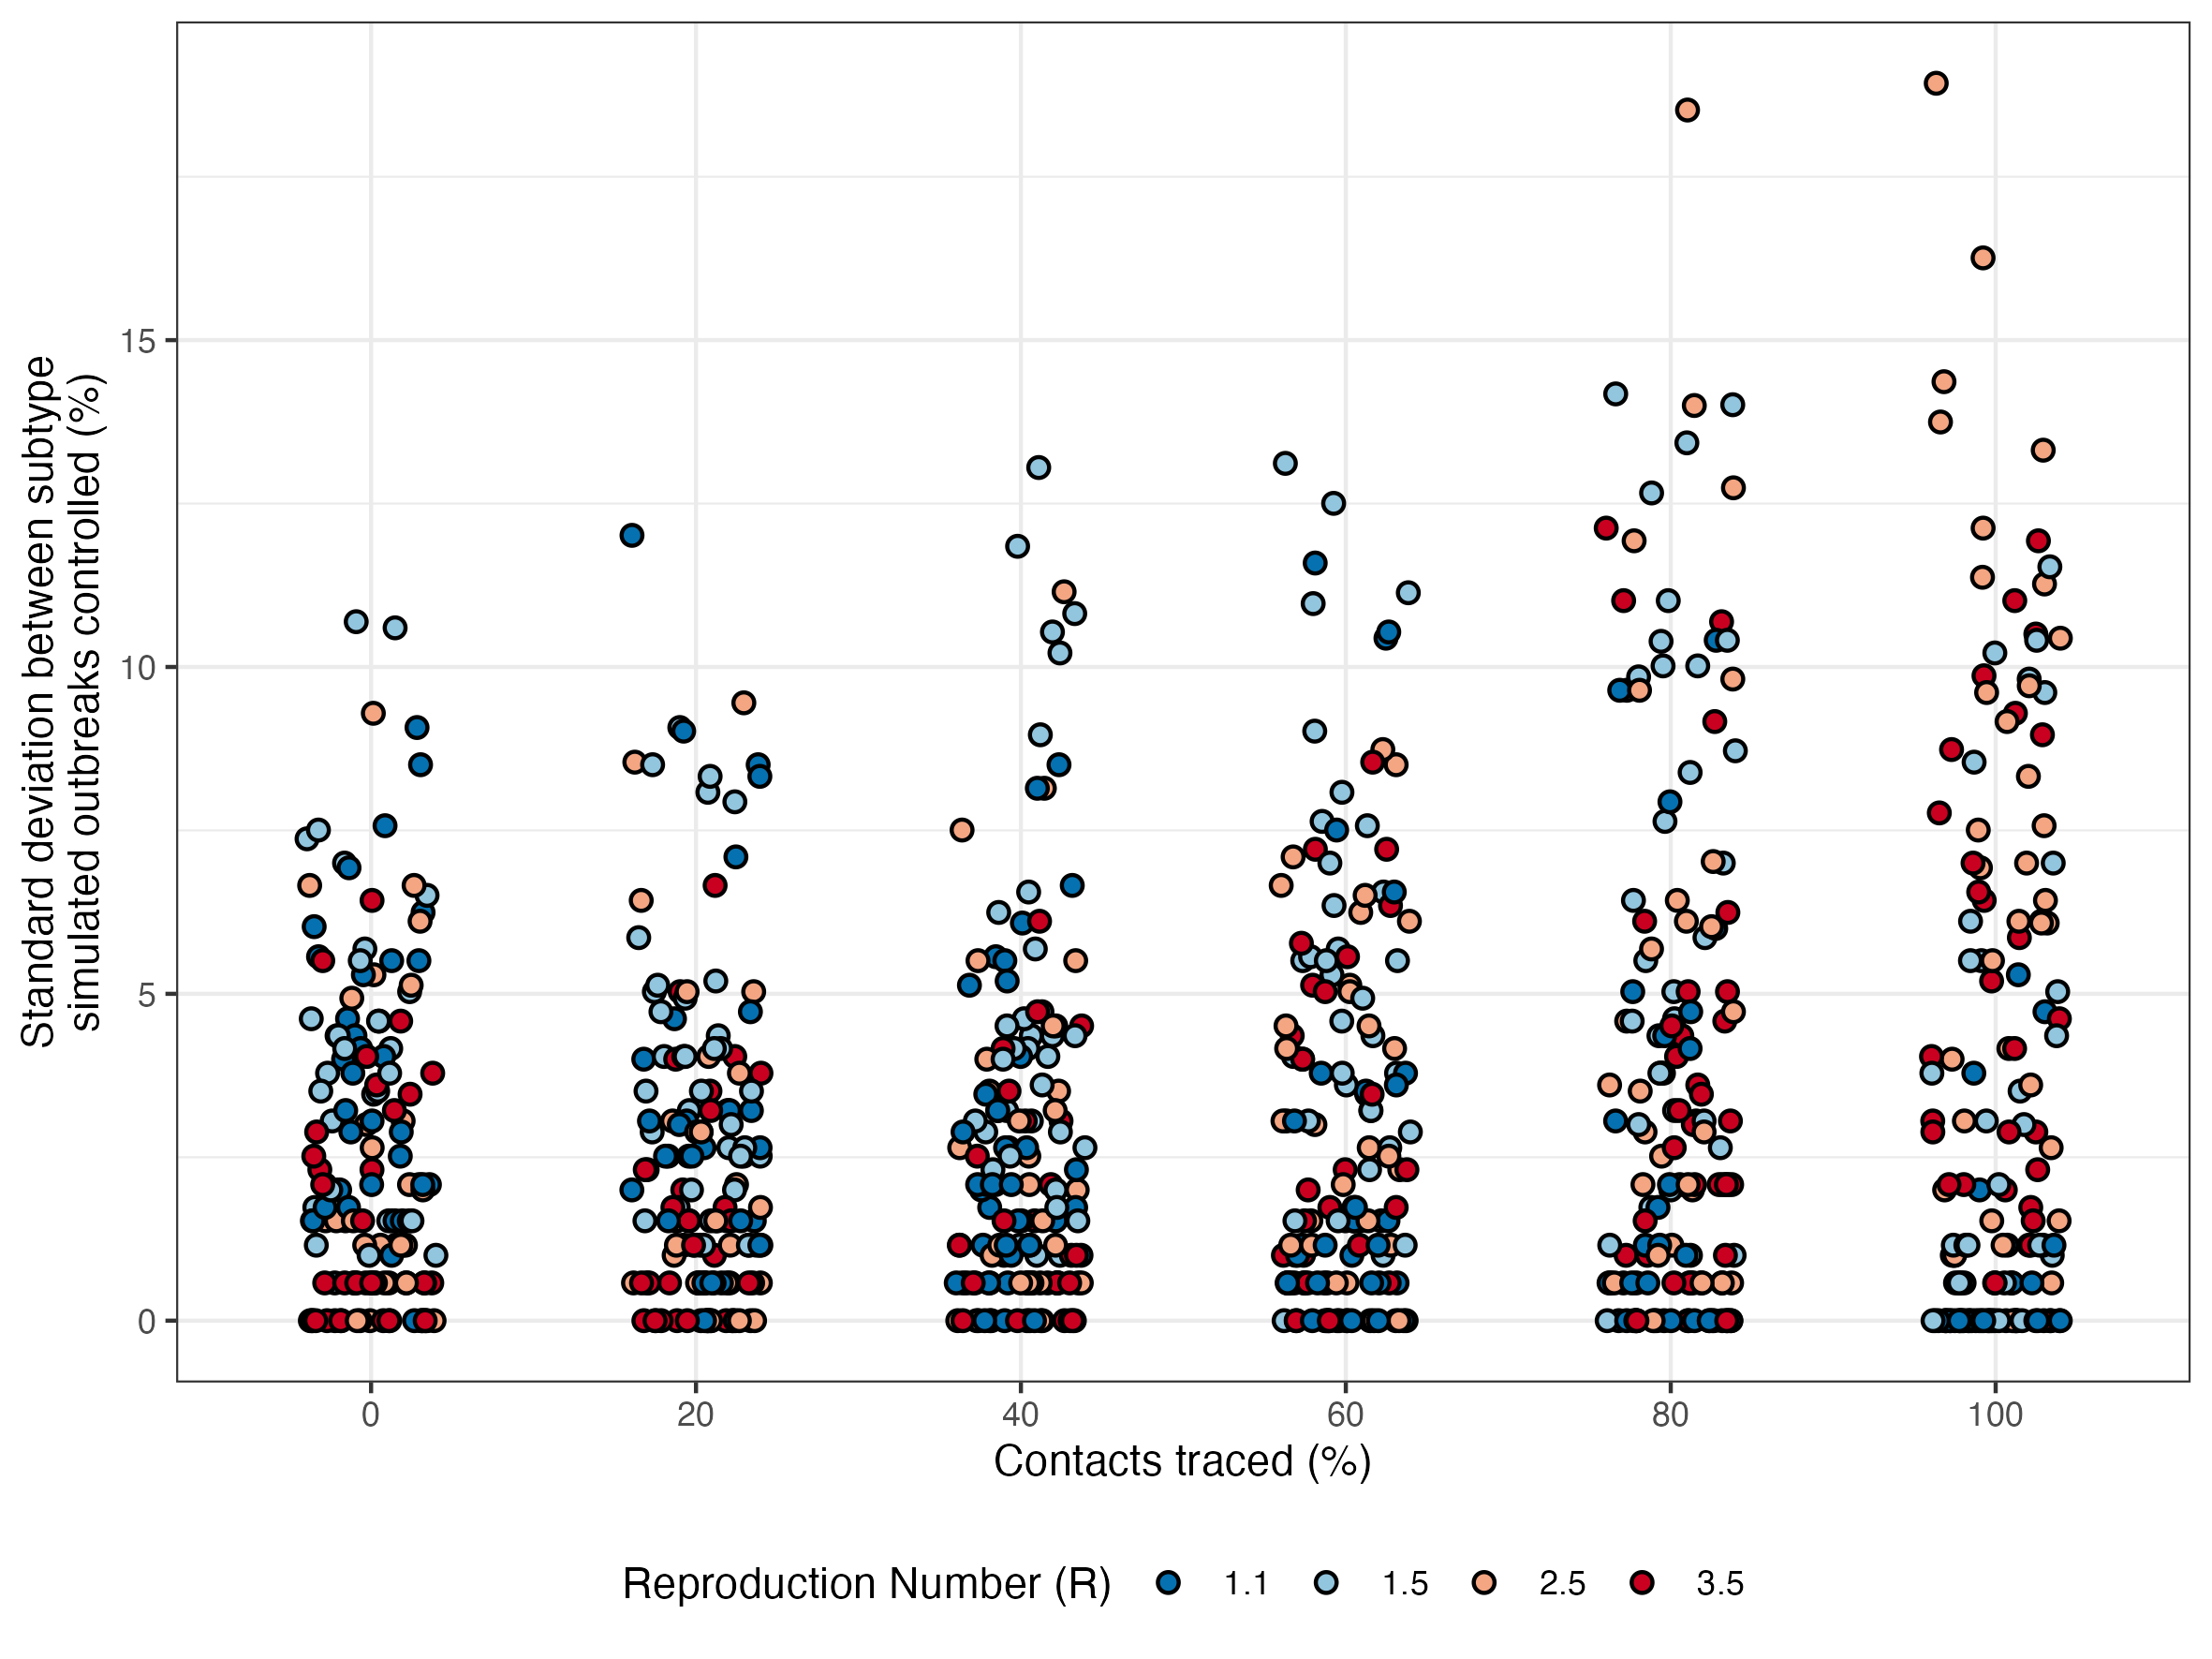
\includegraphics[width=\textwidth]{../plots/prop_outbreak_control_var_reproduction_number.png}
\caption{The standard deviation of the percentage of outbreaks controlled between influenza subtypes (H1N1, H5N1, H7N9), across percentages of contacts traced. Points are jittered horizontally reduce overlap.}
\label{fig:prop-outbreak-control-var-R}
\end{figure}

\begin{figure}[ht]
\centering
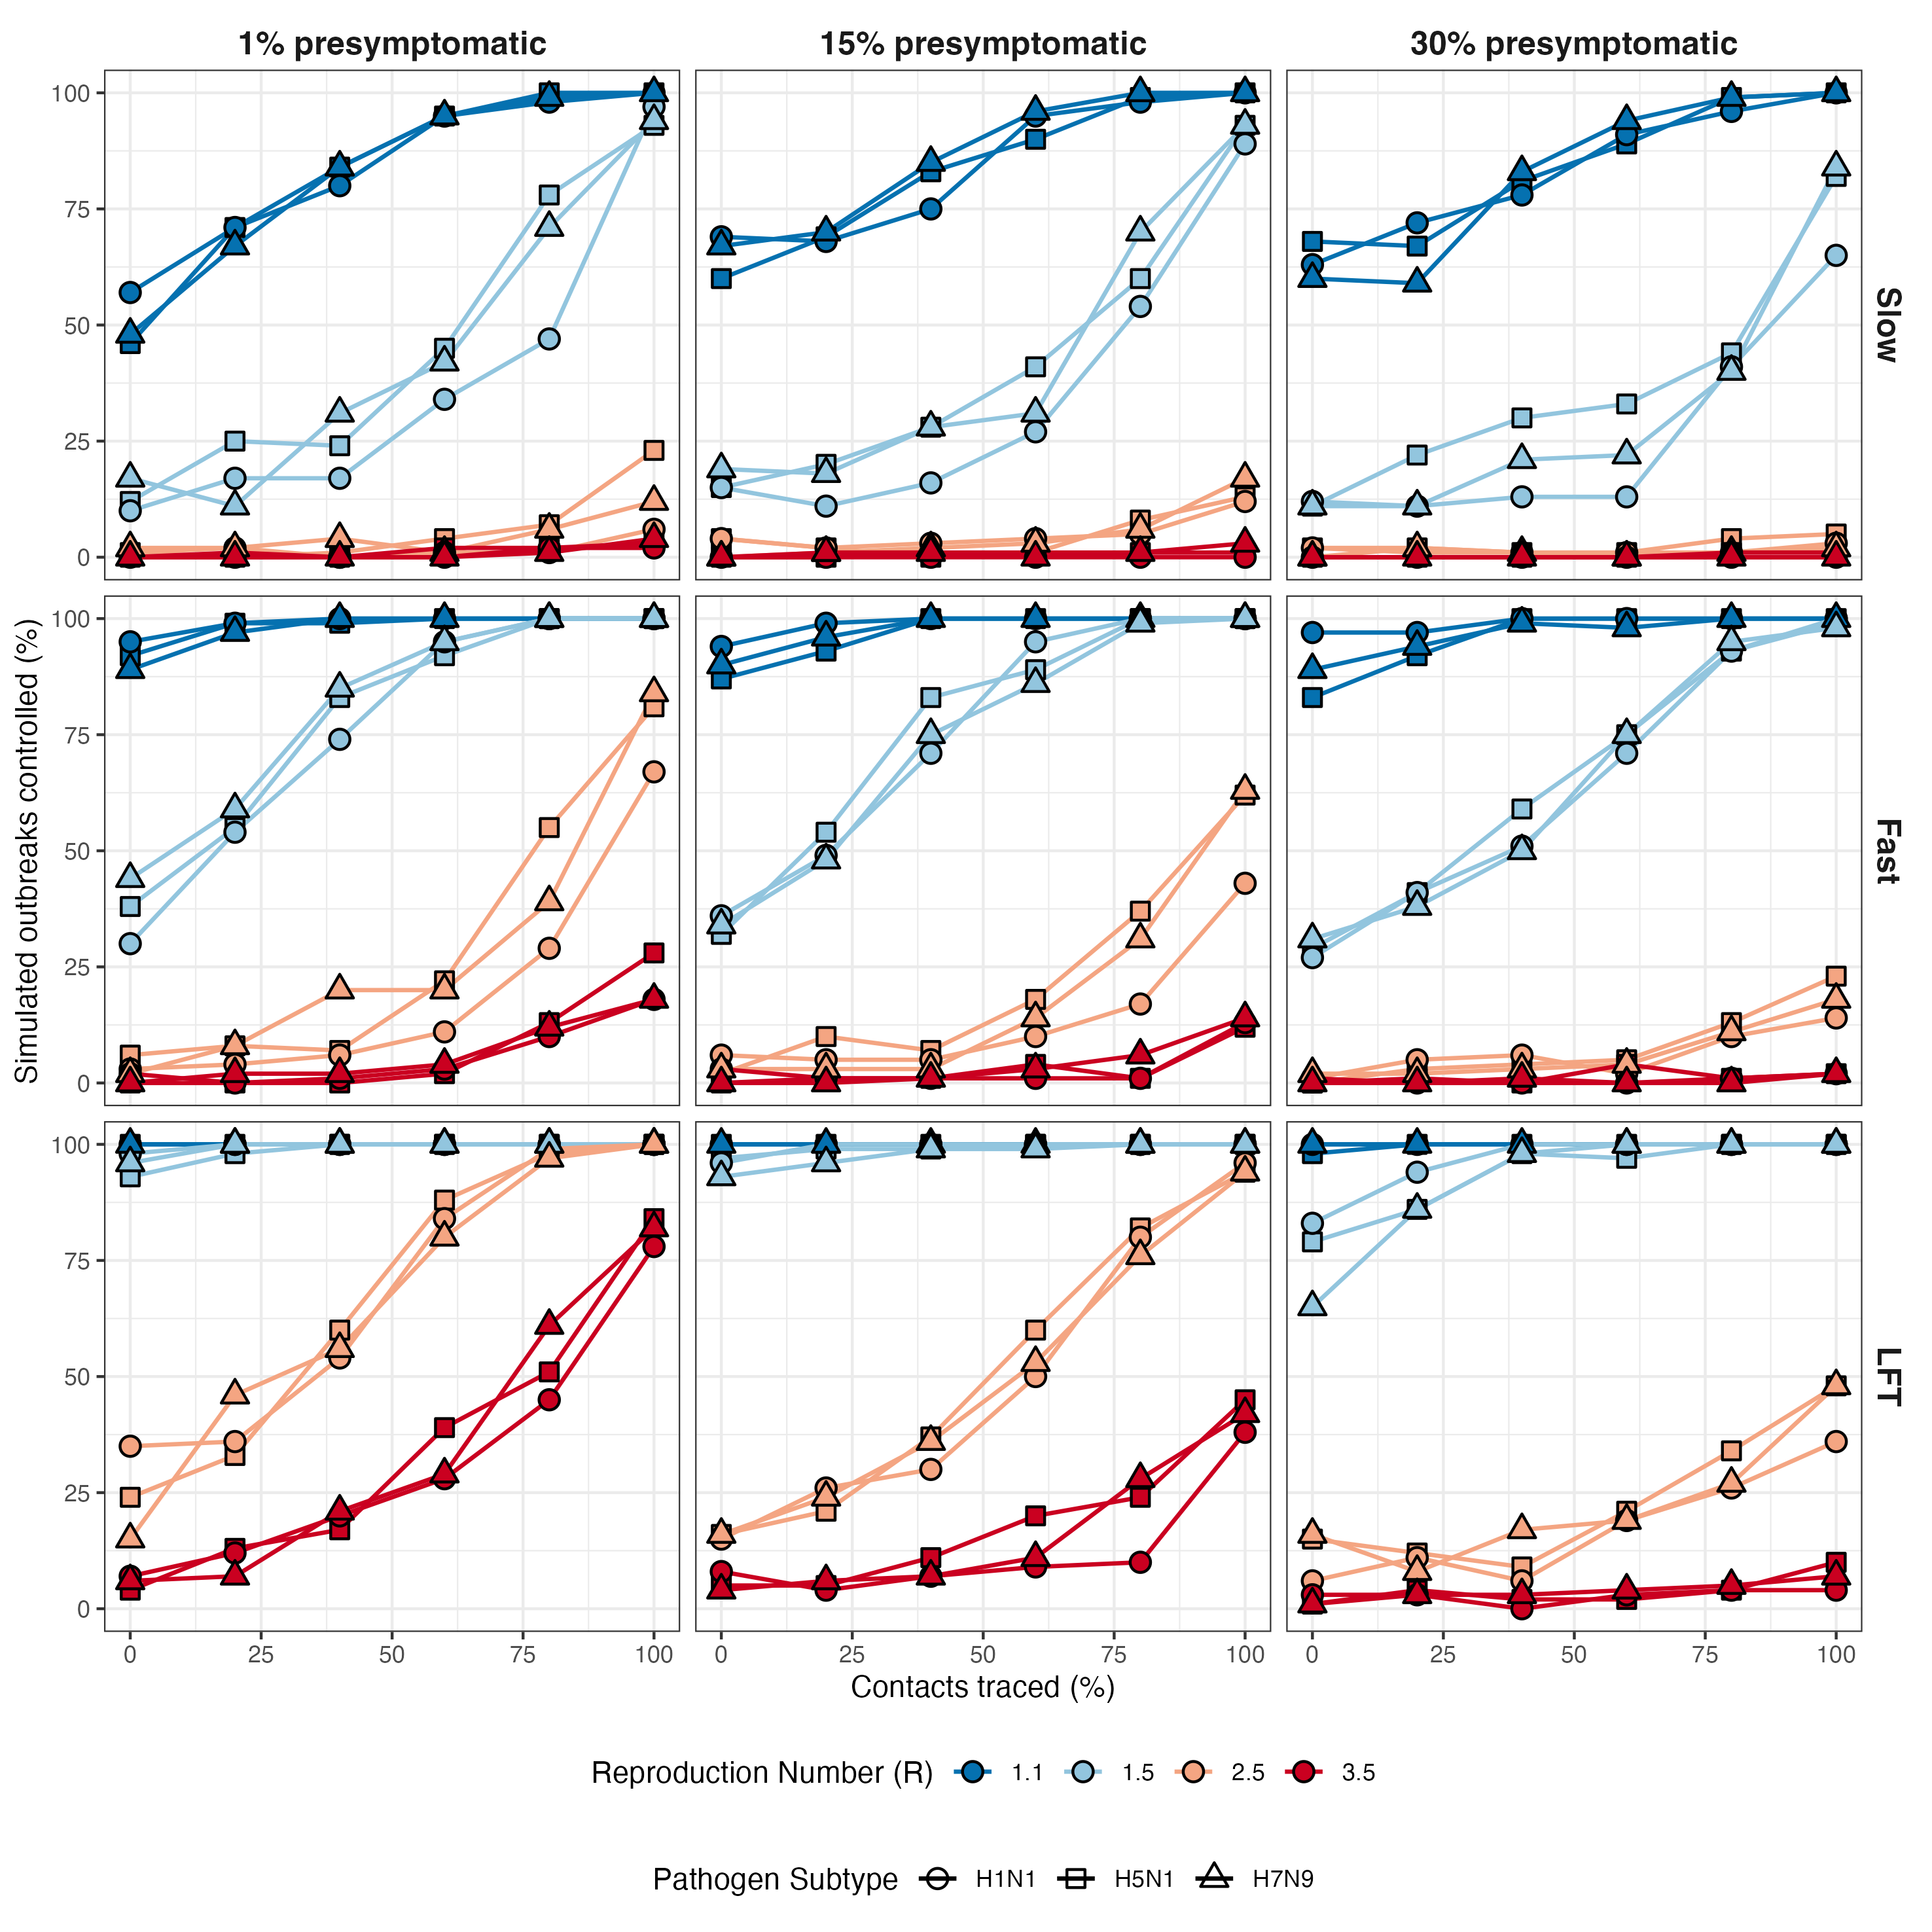
\includegraphics[width=\textwidth]{../plots/prop_outbreak_control_prop_presym_iso.png}
\caption{Stub.}
\label{fig:prop-outbreak-control-prop-presym-iso}
\end{figure}

\begin{figure}[ht]
\centering
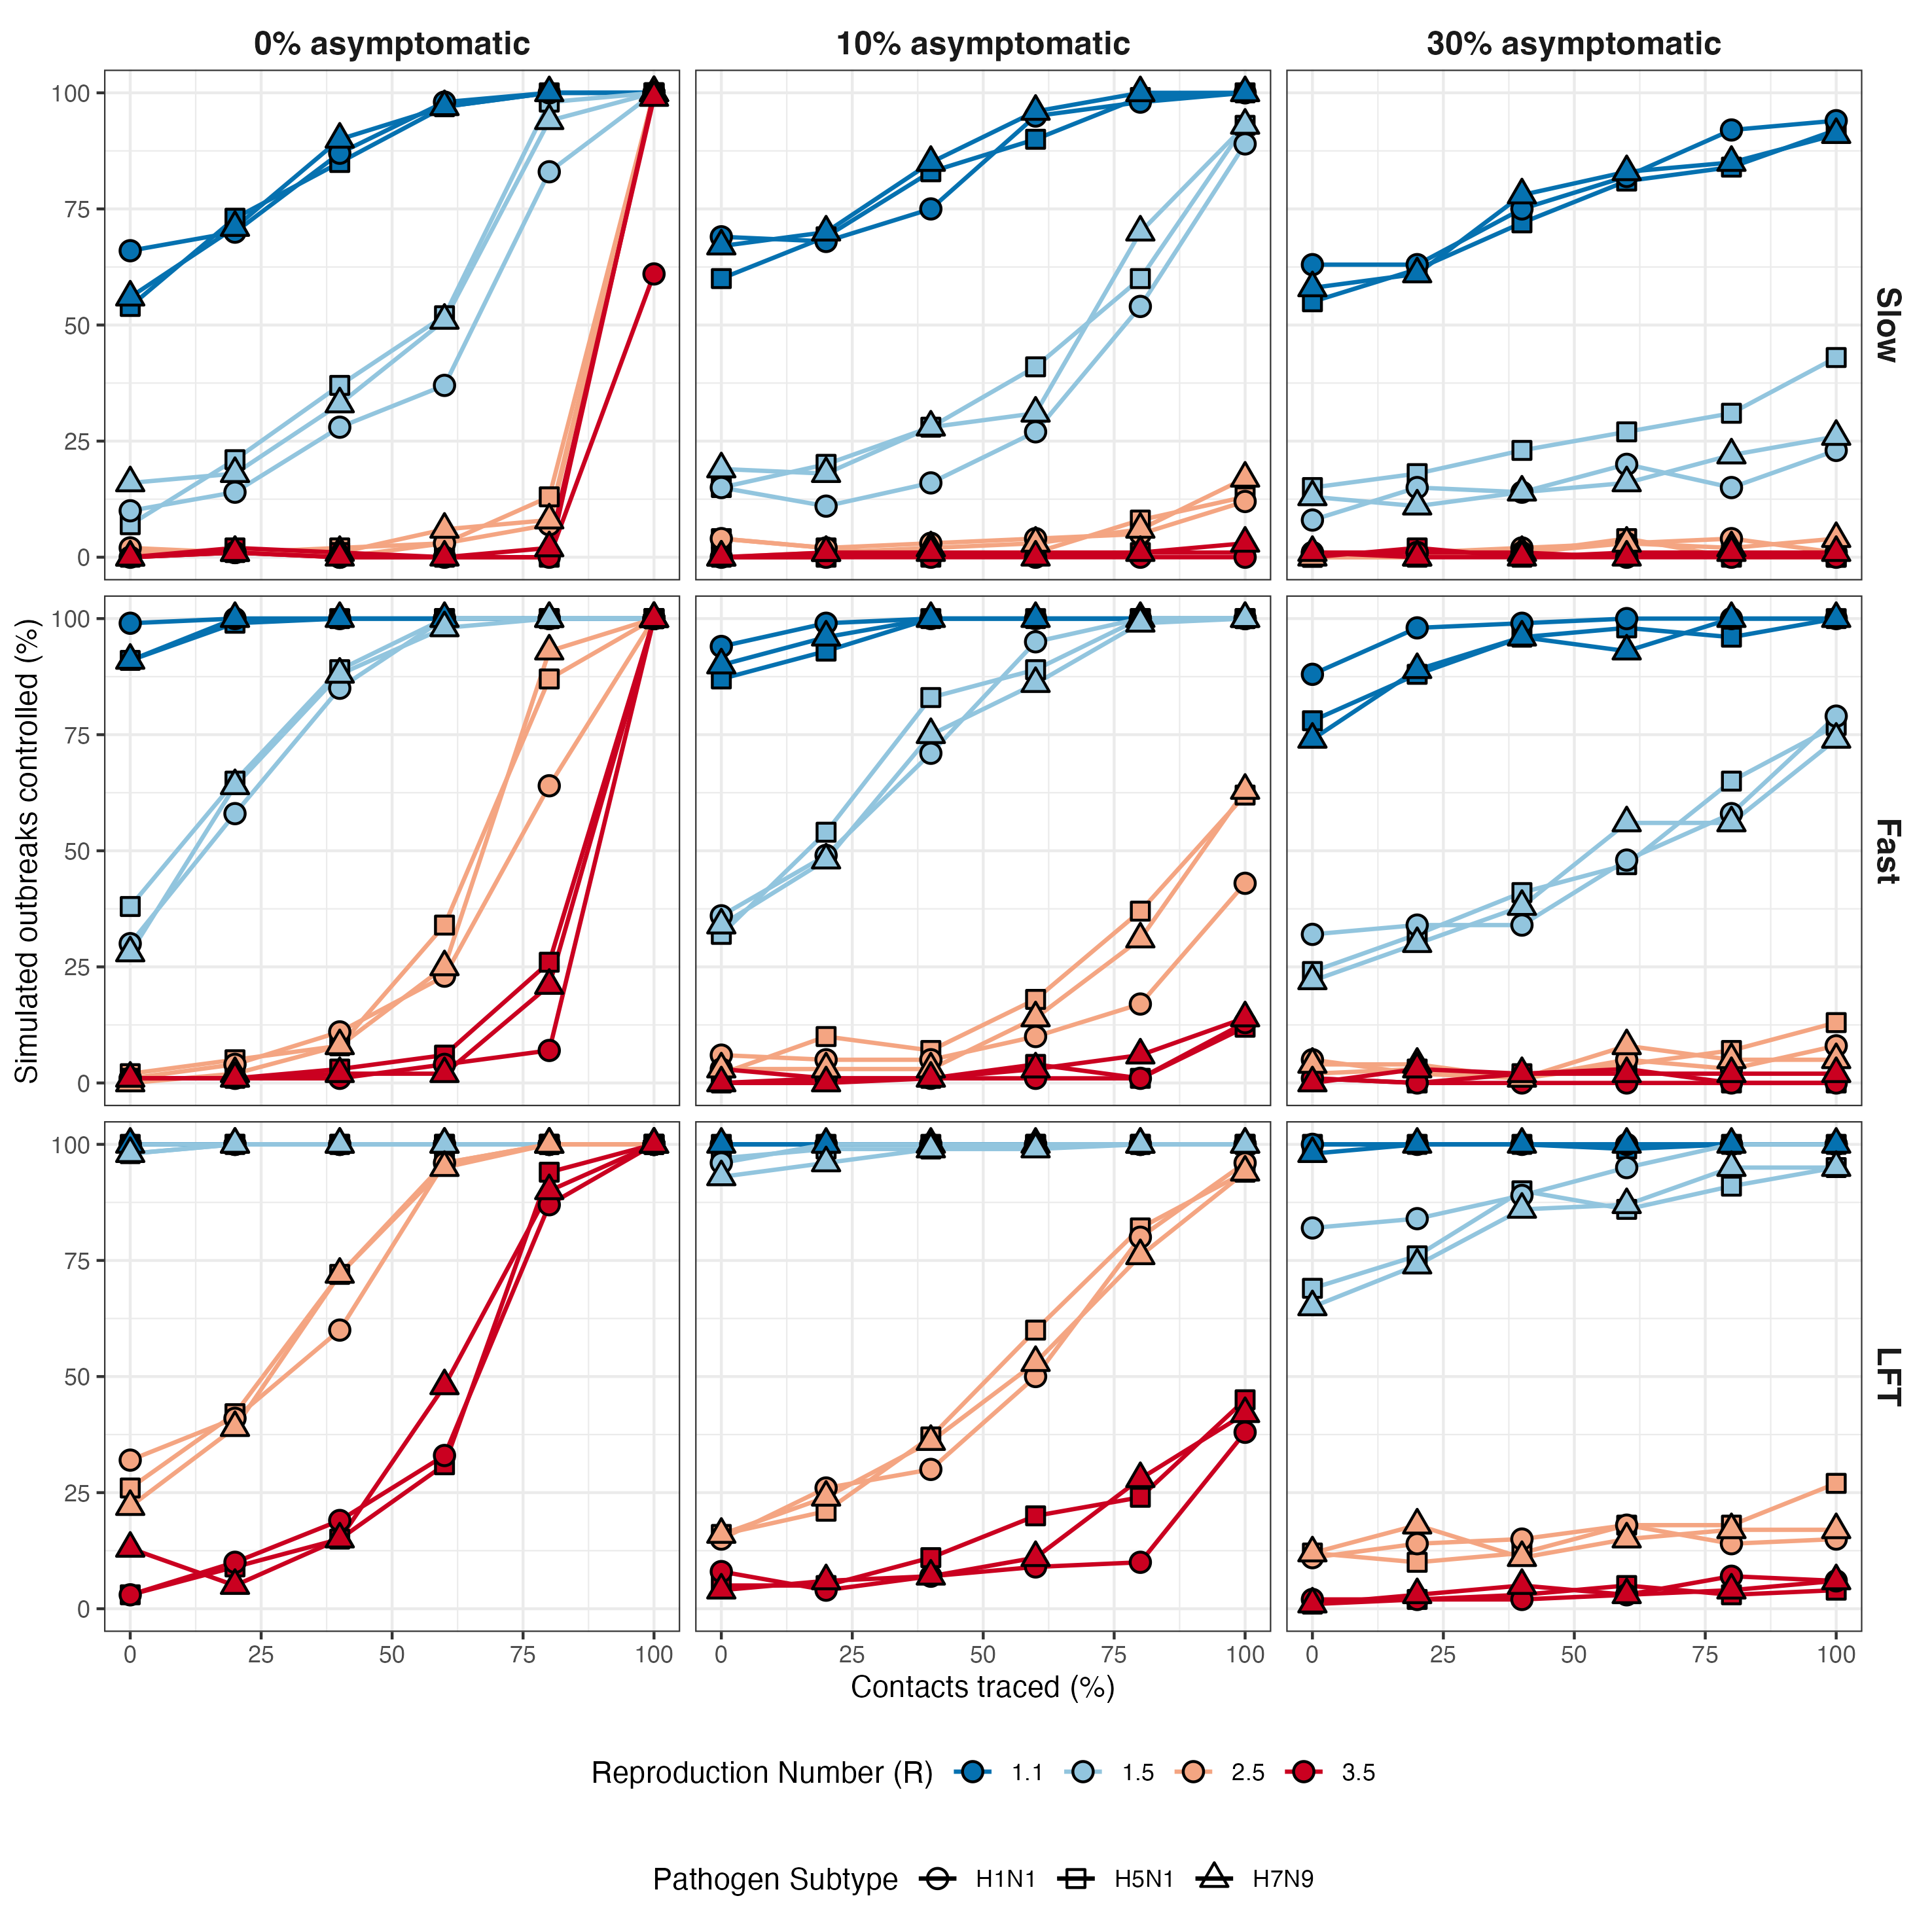
\includegraphics[width=\textwidth]{../plots/prop_outbreak_control_prop_asym_iso.png}
\caption{Stub.}
\label{fig:prop-outbreak-control-prop-asym-iso}
\end{figure}

\begin{figure}[ht]
\centering
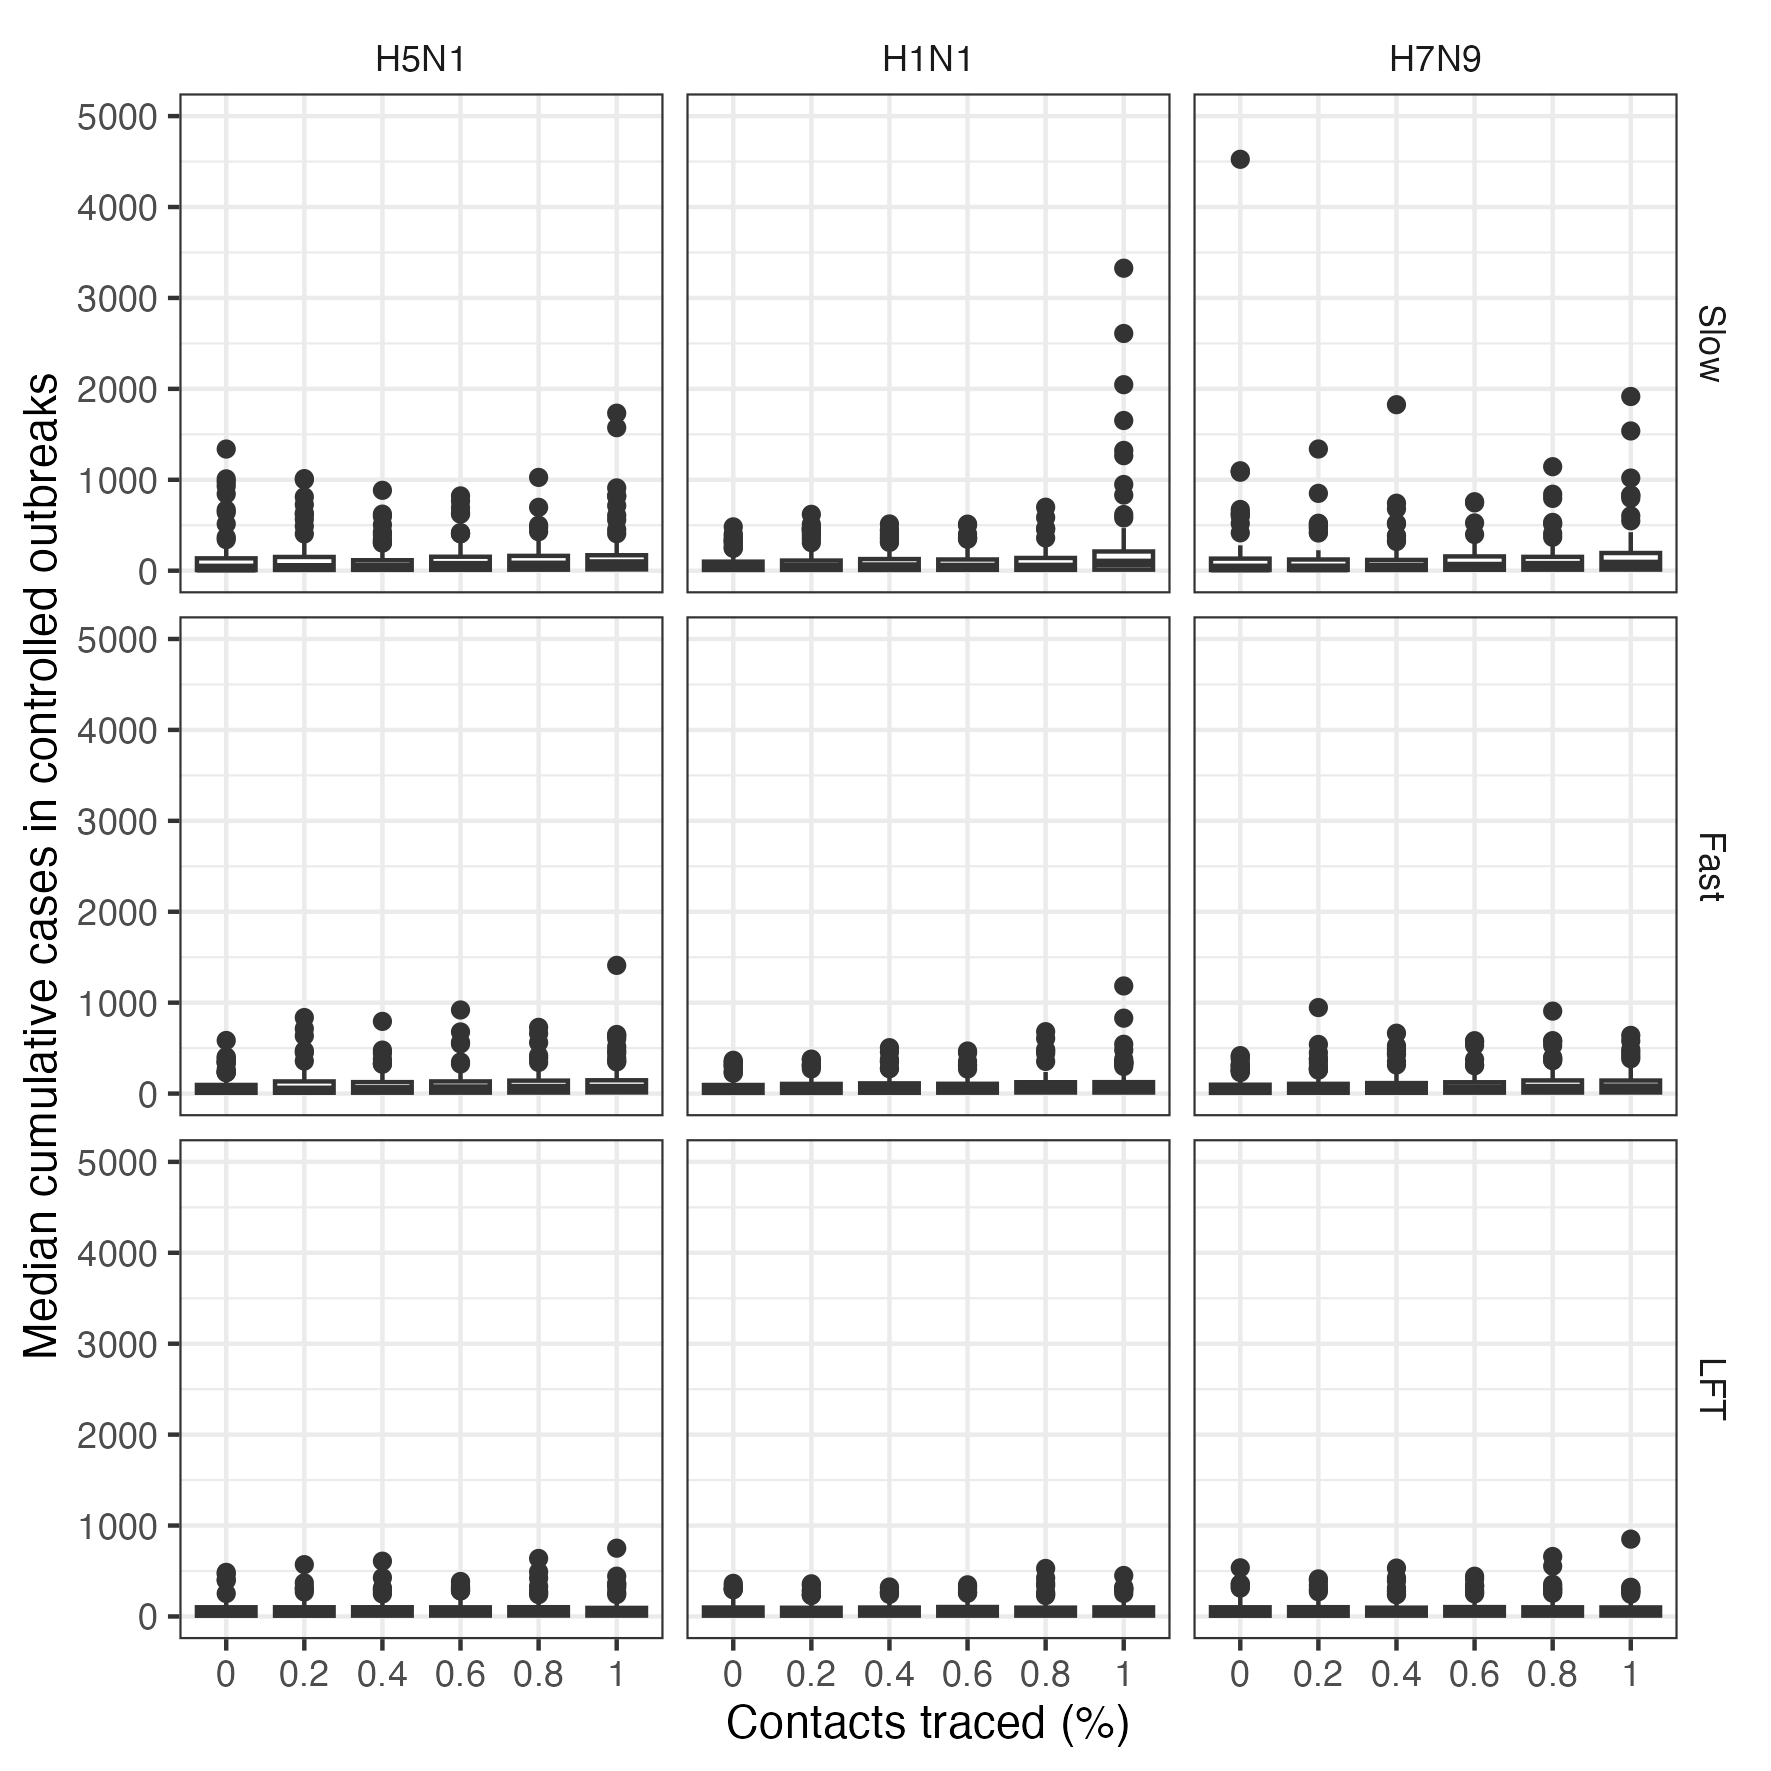
\includegraphics[width=\textwidth]{../plots/median_controlled_outbreak_size.png}
\caption{Median...}
\label{fig:median-controlled-outbreak-size}
\end{figure}

\begin{figure}[ht]
\centering
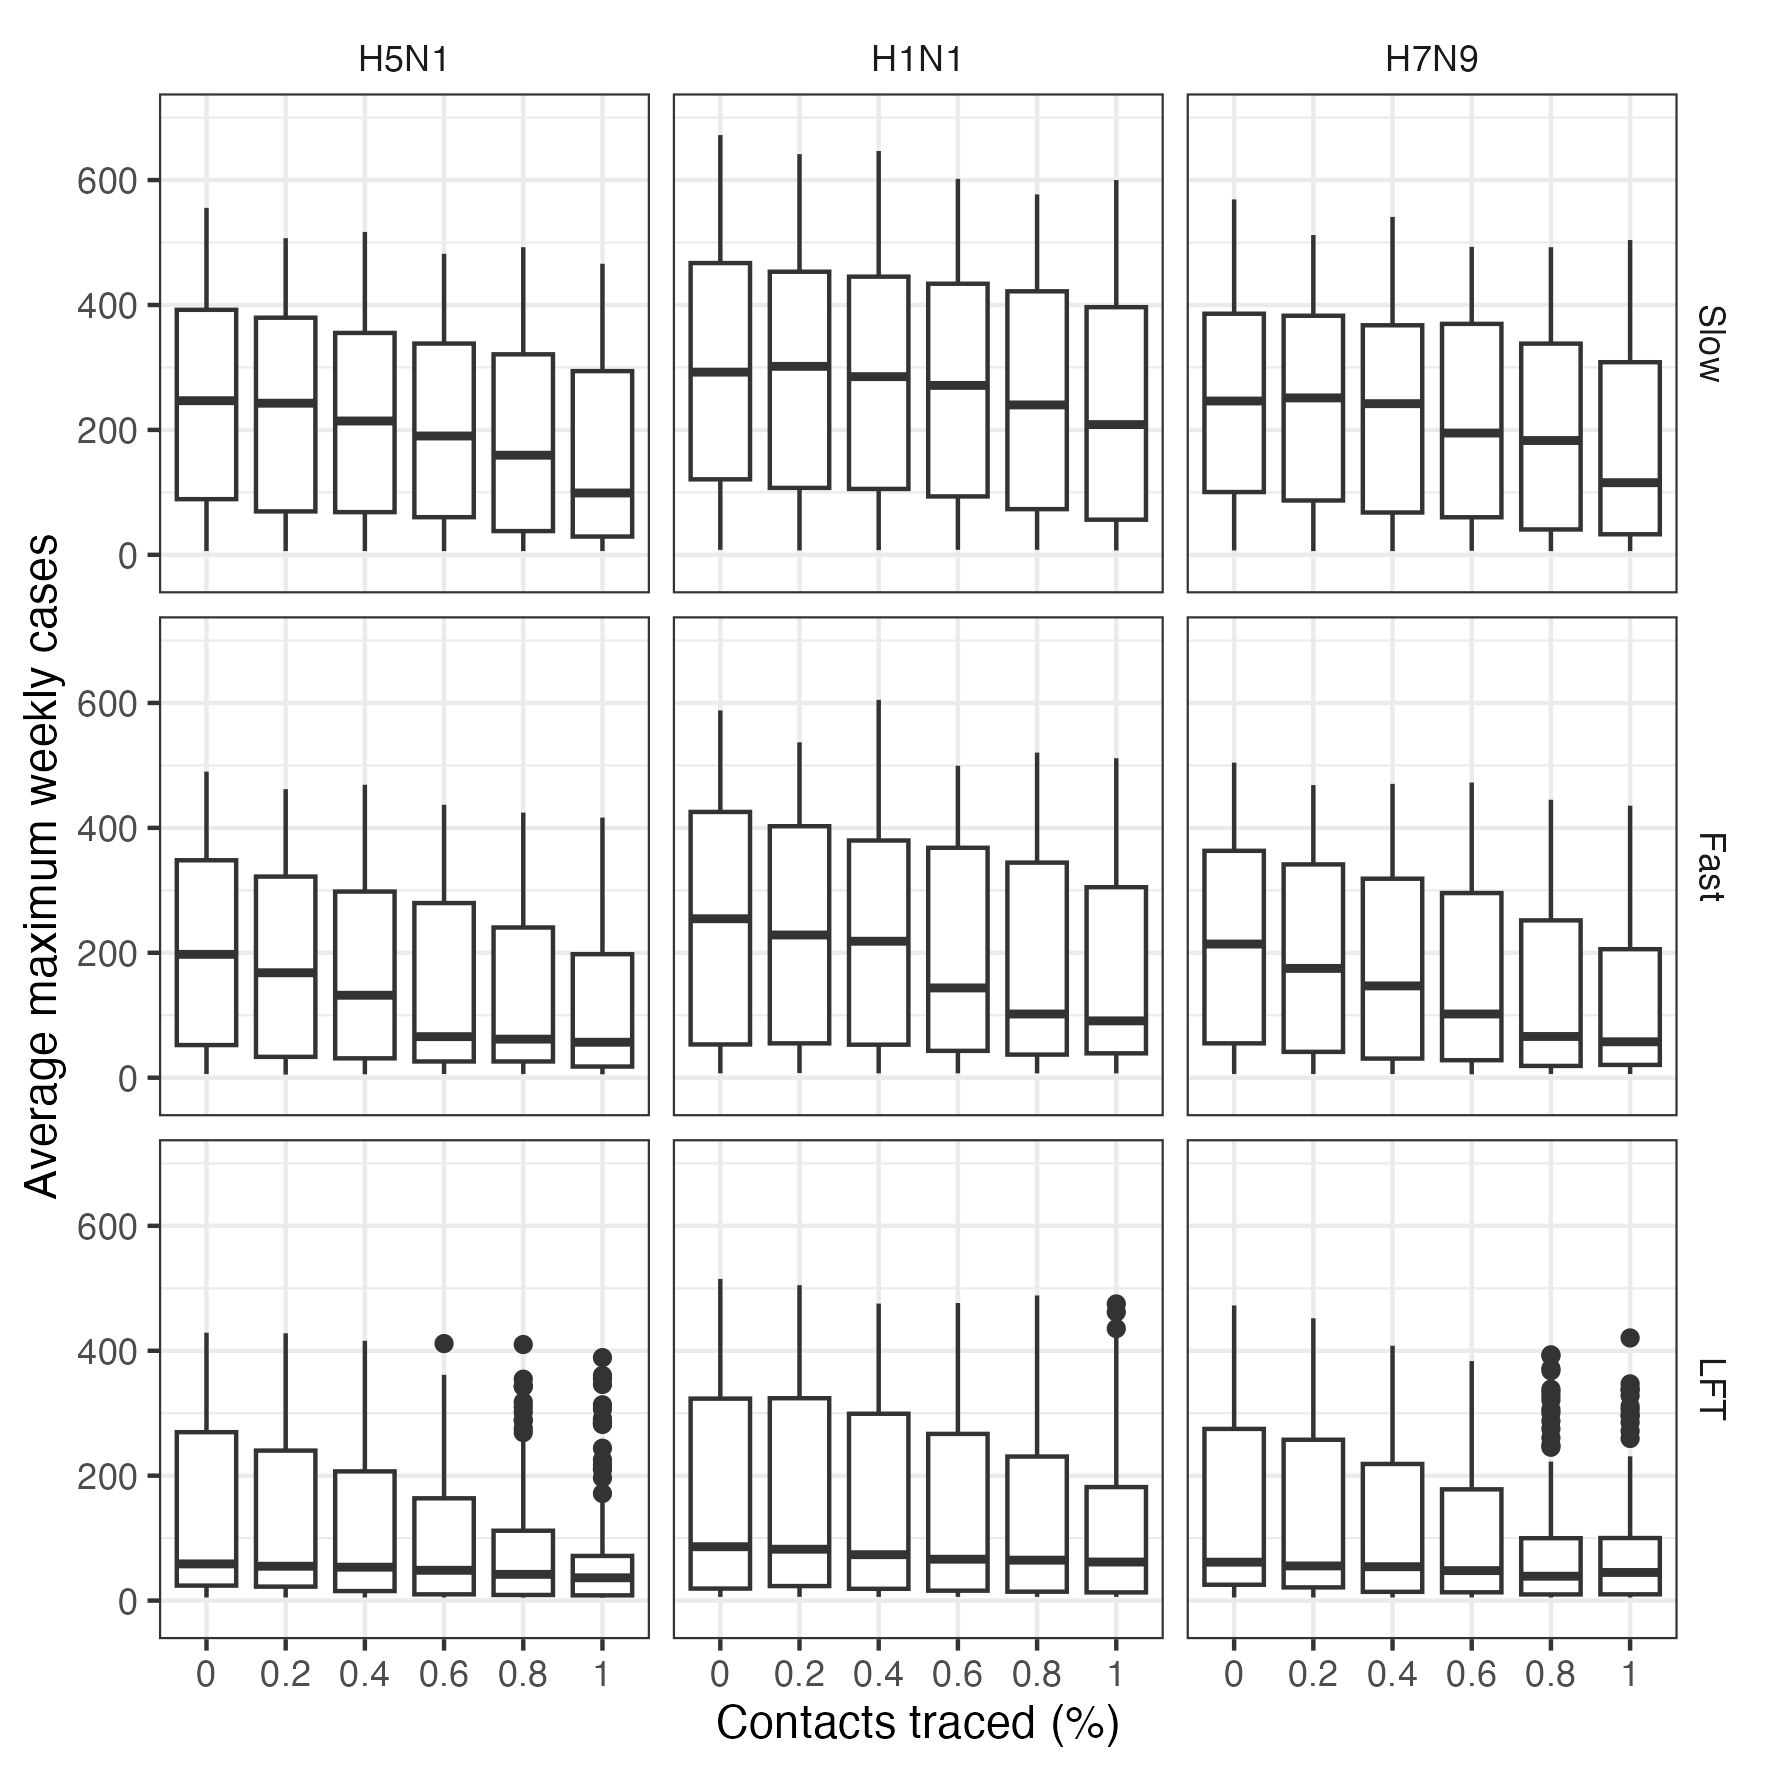
\includegraphics[width=\textwidth]{../plots/max_weekly_cases.png}
\caption{The median maximum number of weekly cases across simulation replicates for different values of community reproduction number ($R_0$). This is facetted by influenza subtype (A/H5N1, A/H1N1, A/H7N9) and onset-to-isolation response delays (slow COVID-like response, fast SARS-like response and LFT self-testing) The boxplots contain all scenarios (e.g., proportion of asymptomatic cases or number of initial cases) within that reproduction number scenario, the whiskers correspond to the 25th and 75th quartiles Data outside of 1.5 $\times$ the interquartile range are plotted as outlier points.}
\label{fig:max-weekly-cases}
\end{figure}

\begin{figure}[ht]
\centering
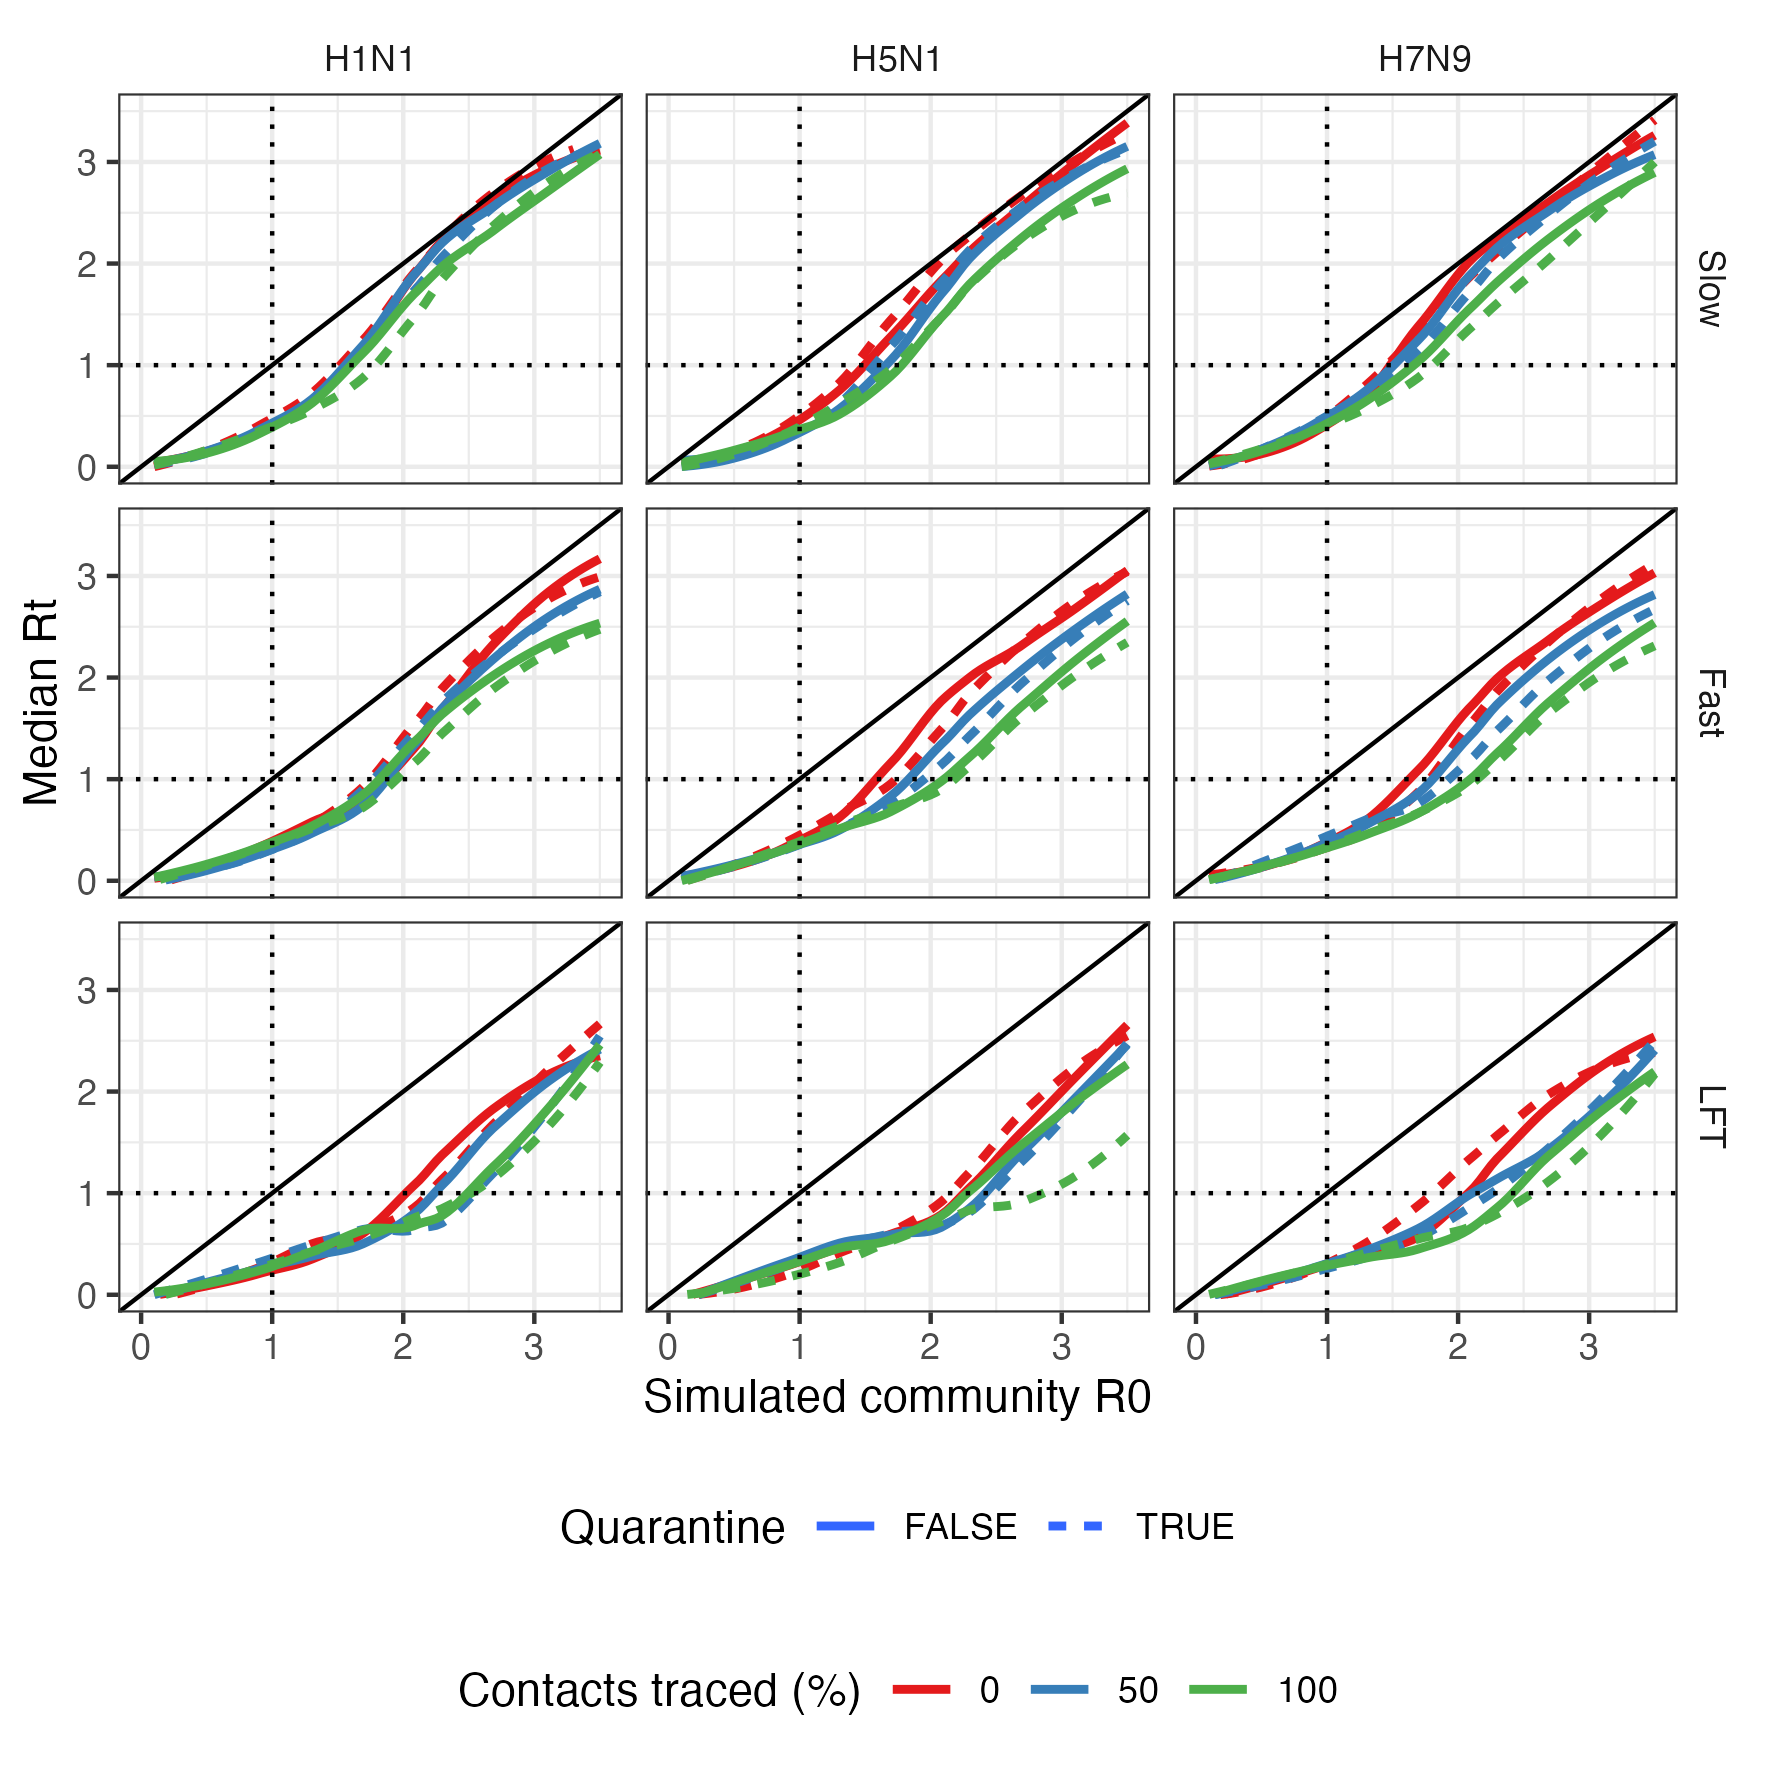
\includegraphics[width=\textwidth]{../plots/r0_high_presym_asym.png}
\caption{The median effective reproduction number ($R_t$) across simulation replicates calculated from simulated outbreak data under various influenza subtype and intervention scenarios against the basic reproduction number ($R_0$) for the general community used to simulate the outbreaks. The $R_0$ value for isolated cases is zero. The diagonal line shows an equal value for $R_t$ and community $R_0$. The dotted lines are where the values of $R_t$ (horizontal) or community $R_0$ (vertical) equal unity. Values of $R_t$ below the diagonal indicate a reduction in transmission from NPIs compared to uncontrolled community transmission. Isolation of symptomatic cases is active for all scenarios, contact tracing ascertainment is plotted for 0\% (no contact tracing), 50\% and 100\% (all symptomatic contacts of symptomatic cases traced), we run each scenario with quarantine of contacts active (dashed line) and inactive (solid line). This is for a baseline scenario where the proportion of presymptomatic transmission is 1\% and the proportion of asymptomatic cases is 0\%.}
\label{fig:r0_high_presym_asym}
\end{figure}

\end{document}
